% main.tex
% Tese de doutorado - Thomas Antonio Cardozo Martins
% Tungstatos de metais de transição aplicados como fotocatalisadores e biocidas

\documentclass[a4paper,12pt]{report}
\usepackage[utf8]{inputenc}
\usepackage[T1]{fontenc}
% Carregar babel uma vez: definir português (Brasil) como idioma principal e inglês como secundário.
% O último idioma na lista de opções se torna o idioma principal do documento.
\usepackage[english,brazil]{babel}
\usepackage{microtype}

% === Pacotes para escrita acadêmica ===
% Matemática e símbolos
\usepackage{amsmath,amssymb,mathtools}
% Quebra automática de equações longas
% O pacote breqn permite que equações longas sejam quebradas automaticamente
% Use \begin{dmath} em vez de \begin{equation} para equações com quebra automática
% Use \begin{dgroup} para grupos de equações com quebra automática
\usepackage{breqn}
% Tratamento melhorado de citações (recomendado com biblatex)
\usepackage{csquotes}

% Gráficos e objetos flutuantes
\usepackage{graphicx}
\usepackage{float}
\usepackage{placeins} % \FloatBarrier

% Tabelas e layout
\usepackage{booktabs}
\usepackage{caption}
\usepackage{subcaption}
\usepackage{enumitem}

% Configurar caption das figuras para ficar no topo
\captionsetup[figure]{position=top}

% Definir comando para fonte da figura (aparece abaixo)
\newcommand{\fonte}[1]{%
  \vspace{0.5\baselineskip}%
  \par\noindent Fonte: #1\par
}

% Configurar espaçamento entre texto e figuras/tabelas
\setlength{\intextsep}{\baselineskip}        % Espaço acima e abaixo de floats no meio do texto
\setlength{\textfloatsep}{\baselineskip}     % Espaço entre floats no topo/fundo da página e texto
\setlength{\floatsep}{\baselineskip}         % Espaço entre floats consecutivos

% Configurar espaçamento fixo de equações: sempre uma linha antes e depois
\makeatletter
% Para subequations: manter uma linha antes
\g@addto@macro\subequations{%
  \setlength{\abovedisplayskip}{\baselineskip}%
  \setlength{\belowdisplayskip}{\baselineskip}%
}
\makeatother

% Ajustar espaçamento para todos os ambientes de equação (equation, align, dmath, etc.)
\AtBeginDocument{%
  \setlength{\abovedisplayskip}{\baselineskip}%
  \setlength{\belowdisplayskip}{\baselineskip}%
  \setlength{\abovedisplayshortskip}{\baselineskip}%
  \setlength{\belowdisplayshortskip}{\baselineskip}%
}

% Unidades e números
\usepackage{siunitx}
\sisetup{detect-all=true, output-decimal-marker={,}}

% Espaçamento, indentação e estrutura do documento
\usepackage{setspace} % \onehalfspacing, \doublespacing
\usepackage{indentfirst} % indentar primeiro parágrafo das seções
\setlength{\parindent}{1.5cm} % Definir indentação de parágrafo globalmente
% fornecer \justifying para justificação completa dentro de minipage
\usepackage{ragged2e}

% Cores e desenho
\usepackage{xcolor}
\usepackage{tikz}
\usepackage{pgfplots}
\pgfplotsset{compat=1.17}

% Notas e marcações editoriais
% Garantir que marginparwidth seja largo o suficiente para todonotes
\setlength{\marginparwidth}{2cm}
\usepackage{todonotes}

% Glossários / acrônimos (requer makeglossaries quando usado)
\usepackage[acronym]{glossaries}
\makeglossaries

% Tabelas longas, notas de tabela e ferramentas extras para tabelas
\usepackage{longtable}
\usepackage{threeparttable}
\usepackage{makecell}

% Pacote para escrever fórmulas químicas
\usepackage[version=4]{mhchem}

% Hiperlinks e referências inteligentes (hyperref deve ser carregado no final)
\usepackage{hyperref}
\usepackage[capitalise,noabbrev]{cleveref}
\hypersetup{
	colorlinks=true,
	linkcolor=black,
	citecolor=black,
	urlcolor=black,
	pdftitle={Tungstatos de metais de transição},
	pdfauthor={Thomas A. C. Martins}
}

% Nota de uso do glossário: para compilar glossários execute `makeglossaries main` após a execução do LaTeX
\usepackage{geometry}
\geometry{a4paper, top=3cm, bottom=2cm, left=3cm, right=2cm}
\usepackage{lipsum}
% Permitir que seções sejam numeradas sem prefixo de capítulo (então seções são 1,2,3... mesmo na classe report)
\usepackage{chngcntr}

% Remover numeração de figuras e tabelas vinculada a capítulos
\counterwithout{figure}{chapter}
\counterwithout{table}{chapter}
\counterwithout{equation}{chapter}
\renewcommand{\thefigure}{\arabic{figure}}
\renewcommand{\thetable}{\arabic{table}}
\renewcommand{\theequation}{\arabic{equation}}

% Configurar profundidade de numeração e sumário para incluir subsubsections
\setcounter{secnumdepth}{3}  % Numerar até subsubsection
\setcounter{tocdepth}{3}      % Incluir subsubsections no sumário

% Fazer cada \section começar em uma nova página
\usepackage{etoolbox}
% Controlar aparência de seção/subseção: manter texto de seção em 12pt, fazer subseção não negrito
\usepackage{titlesec}
% Formatar capítulos: fonte 14, alinhado à esquerda, negrito, com número seguido de ponto
\titleformat{\chapter}
  {\normalfont\fontsize{14}{16}\selectfont\bfseries}
  {\thechapter.}
  {1em}
  {}
% Seções: não negrito, seguindo numeração de capítulo (1.1)
\titleformat{\section}
  {\normalfont\normalsize}
  {\thesection}
  {1em}
  {}
% Subseções: não negrito (1.1.1)
\titleformat{\subsection}
  {\normalfont\normalsize}
  {\thesubsection}
  {1em}
  {}
% Subsubseções: não negrito (1.1.1.1)
\titleformat{\subsubsection}
  {\normalfont\normalsize}
  {\thesubsubsection}
  {1em}
  {}

% Definir numeração de capítulo para usar apenas números
\renewcommand{\thechapter}{\arabic{chapter}}
% Definir numeração de seção como capítulo.seção
\renewcommand{\thesection}{\thechapter.\arabic{section}}
% Definir numeração de subseção como capítulo.seção.subseção
\renewcommand{\thesubsection}{\thesection.\arabic{subsection}}
% Definir numeração de subsubseção como capítulo.seção.subseção.subsubseção
\renewcommand{\thesubsubsection}{\thesubsection.\arabic{subsubsection}}

% Espaçamento: uma linha antes dos títulos (quando após texto ou outro título do mesmo nível), sem espaço após (texto começa imediatamente)
% Capítulo: sem espaço extra
\titlespacing*{\chapter}{0pt}{0pt}{\baselineskip}
% Seção: uma linha antes (quando após texto), uma linha após (para subsection/subsubsection seguinte)
\titlespacing*{\section}{0pt}{\baselineskip}{\baselineskip}
% Subseção: uma linha antes (quando após texto ou outra subsection), sem espaço após
\titlespacing*{\subsection}{0pt}{\baselineskip}{0pt}
% Subsubseção: uma linha antes (quando após texto ou outra subsubsection), sem espaço após
\titlespacing*{\subsubsection}{0pt}{\baselineskip}{0pt}

% Redefinir títulos automáticos removendo a formatação automática e usando manual
\renewcommand{\contentsname}{}
\renewcommand{\listfigurename}{}
\renewcommand{\listtablename}{}

% Garantir que cada \chapter comece em uma página nova adicionando \clearpage antes.
% Isso é feito *depois* que titlesec é carregado para evitar a redefinição de \chapter.
\pretocmd{\chapter}{\clearpage}{}{}

% Seleção de fonte: usar fonte padrão do LaTeX (Computer Modern)
% Comentado: configuração anterior para Arial
% \usepackage{iftex}
% \ifPDFTeX
%   % Fallback pdfLaTeX: usar Helvetica como substituto sans-serif próximo
%   \usepackage[scaled]{helvet}
%   \renewcommand{\familydefault}{\sfdefault}
% \else
%   \usepackage{fontspec}
%   \setmainfont{Arial}
% \fi

% Definir um ambiente `mytext` com tamanho de fonte 12pt,
% espaçamento de linha 1.5 e indentação de parágrafo usando fonte padrão do LaTeX
\usepackage{xparse}
\NewDocumentEnvironment{mytext}{}{
\par\begingroup
	\setstretch{1.5}
	\fontsize{12}{18}\selectfont
	% garantir indentação de parágrafo e parskip modesto
	\setlength{\parindent}{1.25em}
}
{
	\par\endgroup
}

% Definir espaço entre parágrafos padrão como 0pt em todo o documento
\setlength{\parskip}{0pt}

% Bibliografia: usar biblatex-abnt com estilo numérico para formatação ABNT NBR 6023
% Isso segue as regras ABNT mas usa rótulos numéricos [1], [2], ... em vez de autor-ano
\usepackage[backend=biber,style=abnt-numeric,sorting=none,ittitles,uniquename=init,giveninits,justify,indent,repeattitles,sortcites=true,maxbibnames=10,minbibnames=6]{biblatex}
\addbibresource{references.bib}

% Configurar DOI e URL para usar a mesma fonte do texto (não monoespaçada)
\renewcommand*{\mkbibacro}[1]{#1}
\DeclareFieldFormat{doi}{%
  DOI\addcolon\space
  \ifhyperref
    {\href{https://doi.org/#1}{#1}}
    {#1}}
\DeclareFieldFormat{url}{%
  \ifhyperref
    {\href{#1}{#1}}
    {#1}}

% Permitir quebra de linha em URLs e DOIs
\setcounter{biburlnumpenalty}{100}
\setcounter{biburlucpenalty}{100}
\setcounter{biburllcpenalty}{100}

% Configurar quebra de linha para todos os campos bibliográficos
\emergencystretch=1em
\appto{\bibsetup}{\sloppy}

% Adicionar colchetes ao redor dos números de referência na bibliografia
\DeclareFieldFormat{labelnumberwidth}{[#1]}

% Configurar compressão de citações: 
% - 2 referências ou menos: [1, 2]
% - 3 ou mais referências consecutivas: [1-5]
\ExecuteBibliographyOptions{maxcitenames=999}

% Redefinir o comando \cite para usar colchetes únicos com compressão
\DeclareCiteCommand{\cite}[\mkbibbrackets]
  {\usebibmacro{prenote}}
  {\usebibmacro{citeindex}%
   \usebibmacro{cite}}
  {\multicitedelim}
  {\usebibmacro{postnote}}

% Configurar delimitadores para citações múltiplas
\renewcommand*{\multicitedelim}{\addcomma\space}  % Vírgula entre números
\renewcommand*{\compcitedelim}{\textendash}        % Hífen para intervalos (ex: 1-5)

% Configurar limite para compressão: a partir de 3 citações consecutivas
\defbibenvironment{bibliography}
  {\list
     {\printtext[labelnumberwidth]{%
        \printfield{labelprefix}%
        \printfield{labelnumber}}}
     {\setlength{\labelwidth}{\labelnumberwidth}%
      \setlength{\leftmargin}{\labelwidth}%
      \setlength{\labelsep}{\biblabelsep}%
      \addtolength{\leftmargin}{\labelsep}%
      \setlength{\itemsep}{\bibitemsep}%
      \setlength{\parsep}{\bibparsep}}%
      \renewcommand*{\makelabel}[1]{\hss##1}}
  {\endlist}
  {\item}

% Algoritmos e pseudocódigo
\usepackage{algorithm}
\usepackage{algpseudocode}

% Listagens de código (use minted se preferir código com destaque; minted requer -shell-escape)
\usepackage{listings}
% \usepackage{minted} % requer pygments e -shell-escape

% Tipografia para química (se necessário)
\usepackage[version=4]{mhchem}
% pacotes de química intencionalmente omitidos; adicione chemmacros/chemgreek se necessário

% Metadados
\title{TUNGSTATOS DE METAIS DE TRANSIÇÃO APLICADOS COMO
FOTOCATALISADORES E BIOCIDAS: AVALIAÇÃO TEÓRICA DAS ESPÉCIES
REATIVAS DE OXIGÊNIO}
\author{THOMAS ANTONIO CARDOZO MARTINS}
\date{2025y}

% ============================================================
% CONFIGURAÇÃO DE ELEMENTOS PRÉ-TEXTUAIS
% Defina como true ou false para incluir/ocultar cada elemento
% 
% Para INCLUIR um elemento: use \nomedoelemento + true
% Para OCULTAR um elemento: use \nomedoelemento + false
%
% Exemplo:
%   \incluircapatrue         -> Inclui a capa
%   \incluircapafalse        -> Remove a capa do documento
% ============================================================
\newif\ifincluircapa
\newif\ifincluirfolhaderosto
\newif\ifincluirfichacatalografica
\newif\ifincluirfolhadeaprovado
\newif\ifincluirepigrafe
\newif\ifincluiragradecimentos
\newif\ifincluirresumo
\newif\ifincluirabstract
\newif\ifincluirsumario
\newif\ifincluirlistafiguras
\newif\ifincluirlistatabelas
\newif\ifincluirlistaabreviaturas

% Seções principais (true = incluir, false = ocultar)
\newif\ifincluirintroducao
\newif\ifincluirfundamentacao
\newif\ifincluirobjetivos
\newif\ifincluirmetodologia
\newif\ifincluirresultados
\newif\ifincluirconclusao
\newif\ifincluirreferencias
\newif\ifincluirapendice

% Configurar quais elementos serão incluídos (true = incluir, false = ocultar)
\incluircapatrue                   % Capa com logos
\incluirfolhaderostotrue          % Folha de rosto
\incluirfichacatalograficafalse    % Ficha catalográfica (imagem digitalizada)
\incluirfolhadeaprovadofalse       % Folha de aprovação (imagem digitalizada)
\incluirepigrafefalse              % Epígrafe
\incluiragradecimentosfalse        % Agradecimentos
\incluirresumotrue                 % Resumo em português
\incluirabstracttrue               % Abstract em inglês
\incluirsumariotrue                % Sumário (índice)
\incluirlistafigurasfalse          % Lista de figuras
\incluirlistatabelasfalse          % Lista de tabelas
\incluirlistaabreviaturasfalse     % Lista de abreviaturas e siglas

\incluirintroducaotrue             % Capítulo: Introdução
\incluirfundamentacaotrue         % Capítulo: Fundamentação teórica
\incluirobjetivostrue              % Capítulo: Objetivos
\incluirmetodologiatrue            % Capítulo: Metodologia
\incluirresultadostrue             % Capítulo: Resultados e discussão
\incluirconclusaotrue              % Capítulo: Conclusão
\incluirreferenciastrue            % Seção de referências
\incluirapendicefalse              % Apêndice (não numerado no sumário)

\begin{document}

% Usar espaçamento de linha 1.5, comum em documentos acadêmicos
\onehalfspacing
% Garantir que o alinhamento padrão de parágrafo seja totalmente justificado
\justifying

% Pré-textuais (numeração romana)
\pagenumbering{roman}
% Carregar definições do glossário antes das seções pré-textuais
% Defina suas abreviações e acrônimos aqui.
% O glossaries-extra oferece mais opções, mas o glossaries padrão é suficiente para começar.
%
% Formato:
% \newacronym{label}{abreviação}{termo por extenso}
%
% Exemplo:
% \newacronym{dft}{DFT}{Teoria do Funcional da Densidade}
% \newacronym{ros}{ROS}{Espécies Reativas de Oxigênio}

\newacronym{ros}{ROS}{Espécies Reativas de Oxigênio}
\newacronym{dft}{DFT}{Teoria do Funcional da Densidade}

% 0_pre_textuais.tex - páginas pré-textuais (capa, resumo, agradecimentos)

% --- Capa simples (com logos) ---
\ifincluircapa
\begin{titlepage}
  \centering
  \noindent
  \begin{minipage}[t]{0.18\textwidth}
    \raggedright
    \IfFileExists{figures/logo_left.png}{\includegraphics[height=2.2cm]{figures/logo_left.png}}{} % LOGO ESQUERDA
  \end{minipage}%
  \begin{minipage}[t]{0.64\textwidth}
    \centering
    {\large UNIVERSIDADE ESTADUAL DE CAMPINAS\par}
    {\large INSTITUTO DE QUÍMICA\par}
  \end{minipage}%
  \begin{minipage}[t]{0.18\textwidth}
    \raggedleft
    \IfFileExists{figures/logo_right.png}{\includegraphics[height=2.2cm]{figures/logo_right.png}}{} % LOGO DIREITA
  \end{minipage}

  \vspace{4cm}
  {\large THOMAS ANTONIO CARDOZO MARTINS\par}

  \vspace*{4cm}

  {\large TUNGSTATOS DE METAIS DE TRANSIÇÃO APLICADOS COMO FOTOCATALISADORES E BIOCIDAS: AVALIAÇÃO TEÓRICA DAS ESPÉCIES REATIVAS DE OXIGÊNIO\par}

  \vspace*{\fill}
  {\large CAMPINAS\par}
  {\large \the\year\par} % ano atual automático
\end{titlepage}
\fi

% --- Folha de rosto ---
\ifincluirfolhaderosto
\begin{titlepage}
  \centering
   {\large THOMAS ANTONIO CARDOZO MARTINS\par}
    \vspace*{9cm}
   {\large TUNGSTATOS DE METAIS DE TRANSIÇÃO APLICADOS COMO FOTOCATALISADORES E BIOCIDAS: AVALIAÇÃO TEÓRICA DAS ESPÉCIES REATIVAS DE OXIGÊNIO\par}
    \vspace*{2cm}
    % Position the paragraph so its left edge starts at the horizontal center of the page
   \noindent\hspace*{0.5\textwidth}\begin{minipage}[t]{0.5\textwidth}
     \raggedright
     \justifying
      {\noindent Exame de qualificação geral de doutorado apresentada ao Programa de Pós-Graduação em Química, Instituto de Química, Universidade Estadual de Campinas, como requisito parcial à obtenção do título de Doutor em Química.}
        \par\vspace{0.5\baselineskip}
      {\noindent Orientador: Miguel Angel San-Miguel Barrera}\par
         \par\vspace{0.5\baselineskip}
      %{\noindent Coorientador: Juan Andrés}\par
    \end{minipage}

  \vspace*{\fill}
  {\large CAMPINAS\par}
  {\large \the\year\par}
\end{titlepage}
\fi


% --- Ficha Catalográfica ---
\ifincluirfichacatalografica
\clearpage
\thispagestyle{empty}
\vspace*{\fill}
\begin{center}
  \IfFileExists{figures/ficha_catalografica.pdf}{%
    \includegraphics[width=\textwidth,height=\textheight]{figures/ficha_catalografica.pdf}
  }{%
    \IfFileExists{figures/ficha_catalografica.png}{%
      \includegraphics[width=\textwidth,height=\textheight]{figures/ficha_catalografica.png}
    }{%
      % Caso a imagem não exista, exibir mensagem
      \vspace*{3cm}
      {\large \textbf{FICHA CATALOGRÁFICA}\par}
      \vspace{1cm}
      {\normalsize [Insira aqui a imagem digitalizada da ficha catalográfica]\par}
      \vspace{1cm}
      {\small Arquivo esperado: figures/ficha\_catalografica.pdf ou figures/ficha\_catalografica.png\par}
    }%
  }%
\end{center}
\vspace*{\fill}
\fi


% --- Folha de Aprovação ---
\ifincluirfolhadeaprovado
\clearpage
\begin{center}
  \thispagestyle{empty}
  \vspace*{\fill}
  \IfFileExists{figures/folha_aprovacao.pdf}{%
    \includegraphics[width=\textwidth,height=0.95\textheight,keepaspectratio]{figures/folha_aprovacao.pdf}
  }{%
    \IfFileExists{figures/folha_aprovacao.png}{%
      \includegraphics[width=\textwidth,height=0.95\textheight,keepaspectratio]{figures/folha_aprovacao.png}
    }{%
      % Caso a imagem não exista, exibir mensagem
      \vspace*{3cm}
      {\large \textbf{FOLHA DE APROVAÇÃO}\par}
      \vspace{1cm}
      {\normalsize [Insira aqui a imagem digitalizada da folha de aprovação]\par}
      \vspace{1cm}
      {\small Arquivo esperado: figures/folha\_aprovacao.pdf ou figures/folha\_aprovacao.png\par}
    }%
  }%
  \vspace*{\fill}
\end{center}
\fi

% --- Epígrafe ---
\ifincluirepigrafe
\clearpage
\vspace*{\fill}
\begin{flushright}
  Epígrafe - lerolerolerolerolerolero
\end{flushright}
\fi


% --- Agradecimentos (opcional) ---
\ifincluiragradecimentos
\clearpage
\begin{center}
\fontsize{14}{16}\selectfont\textbf{AGRADECIMENTOS}
\end{center}

\begin{text}
  Ao meu orientador prof. Dr. Miguel Angel San-Miguel Barrera...

  Ao meu coorientador prof. Dr. Juan Andrés...
\end{text}
\fi

% --- Resumo (em português) ---
\ifincluirresumo
\clearpage
\begin{center}
  \fontsize{14}{16}\selectfont\textbf{Resumo}
\end{center}
\begin{text}
    \noindent Espécies reativas de oxigênio (ROS), como superóxidos ($^\bullet$O$_{\text{2}}^{-}$) e radicais hidroxila ($^{\bullet}$OH), desempenham papel central na eliminação de patógenos e células cancerígenas no meio biológico, despertando crescente interesse na sua geração controlada para aplicações em saúde. Semicondutores destacam-se como materiais promissores para esse fim, pois permitem a formação fotocatalítica de ROS a partir de moléculas de H$_{\text{2}}$O e O$_{\text{2}}$ adsorvidas em suas superfícies. Assim, o desenvolvimento de novos semicondutores, com propriedades estruturais e eletrônicas otimizadas, é essencial para aprimorar sua eficiência fotocatalítica. Entre esses materiais, os tungstatos metálicos (M$_{\text{x}}$WO$_{\text{4}}$) apresentam desempenho promissor e relevância estratégica no Brasil, que possui reservas minerais significativas no estado do Rio Grande do Norte. Contudo, abordagens exclusivamente experimentais podem ser limitadas para o estudo aprofundado de suas propriedades eletrônicas. Nesse contexto, métodos teóricos baseados em química computacional oferecem uma abordagem eficazes para investigar, em nível atômico, suas características estruturais, eletrônicas e morfológicas dos materiais. Este projeto propõe o uso da Teoria do Funcional da Densidade (DFT) e de Dinâmica Molecular Quântica para estudar tungstatos metálicos (ZnWO$_{\text{4}}$, NiWO$_{\text{4}}$ e CoWO$_{\text{4}}$), avaliando o efeito do cátion modificador da rede sobre suas propriedades e sua capacidade de adsorver H$_{\text{2}}$O e O$_{\text{2}}$, visando compreender os mecanismos de geração de ROS e sua potencial atividade bactericida.
    
    \vspace{1em}    
    \noindent \textbf{Palavras-chave:} Tungstatos; ROS; Química computacional; Fotocatálise.
\end{text}
\fi

% --- Abstract ---
\ifincluirabstract
\clearpage
\begin{center}
  \fontsize{14}{16}\selectfont\textbf{ABSTRACT}
\end{center}
  \begin{text}
  \noindent Reactive oxygen species (ROS), such as superoxide ($^{\bullet}$O$_2^{-}$) and hydroxyl radicals ($^{\bullet}$OH), play a central role in eliminating pathogens and cancer cells in biological systems, generating increasing interest in their controlled production for healthcare applications. Semiconductors stand out as promising materials for this purpose, as they enable the photocatalytic formation of ROS from H$_{\text{2}}$O and O$_{\text{2}}$ molecules adsorbed on their surfaces. Therefore, the development of novel semiconductors with optimized structural and electronic properties is essential to enhance their photocatalytic efficiency. Among these materials, metal tungstates (M$_{\text{x}}$WO$_{\text{4}}$) exhibit promising performance and strategic relevance in Brazil, which holds significant mineral reserves in the state of Rio Grande do Norte. However, purely experimental approaches may be limited in providing an in-depth understanding of their electronic properties. In this context, theoretical methods based on computational chemistry provide an effective approach to investigate, at the atomic level, their structural, electronic, and morphological properties of materials.tungstates (ZnWO$_{\text{4}}$, NiWO$_{\text{4}}$, and CoWO$_{\text{4}}$), evaluating the effect of the network-modifying cation on their properties and their ability to adsorb H$_{\text{2}}$O and O$_{\text{2}}$, with the goal of elucidating the mechanisms of ROS generation and their potential bactericidal activity. 

  \vspace{1em}
  \noindent \textbf{Keywords:} Tungstates; ROS; Computational chemistry; Photocatalysis.
\end{text}
\fi

% --- Sumário ---
\ifincluirsumario
\tableofcontents
\fi

% --- Lista de Figuras ---
\ifincluirlistafiguras
\listoffigures
\fi

% --- Lista de Tabelas ---
\ifincluirlistatabelas

\listoftables
\fi

% --- Lista de Abreviaturas e Siglas ---
\ifincluirlistaabreviaturas
\printglossary[type=\acronymtype, title={}]
\fi



\clearpage
% Conteúdo principal (numeração arábica continuando da romana)
% Salvar o contador de páginas atual
\newcounter{preTextualPages}
\setcounter{preTextualPages}{\value{page}}
\pagenumbering{arabic}
% Continuar a numeração da parte pré-textual
\setcounter{page}{\value{preTextualPages}}

\ifincluirintroducao
% 1_introducao.tex
\chapter{INTRODUÇÃO}

Espécies reativas de oxigênio (ROS, do inglês reactive oxygen species) são um grupo de moléculas oxigenadas derivadas de oxigênio molecular e da água que englobam espécies radicalares como ânion superóxido ($^{\bullet}$O$_{2}^{-}$), radical hidroxila ($^{\bullet}$OH) e hidroperoxila ($^{\bullet}$O$_{2}$H). Além disso, algumas espécies não radicalares que são facilmente convertidas em radicais como peróxido de hidrogênio (H$_{2}$O$_{2}$) e oxigênio singleto ($^{1}$O$_{2}$) também fazem parte desse grupo \cite{bayr2005reactive,dong2022comprehensive}. A formação dessas espécies radicalares e não radicalares ocorre em ambientes oxidantes dentro das células durante processos aeróbicos de metabolismo, seja em condições normais ou de estresse \cite{Sachdev2023}. Essas espécies se originam do oxigênio molecular e da água, como pode ser observado na Figura \ref{fig:ros_formation} que esquematiza a formação das principais espécies.

\begin{figure}[htbp]
  \caption{Esquema da formação das principais espécies reativas de oxigênio (ROS) a partir do oxigênio molecular e da água.}
  \label{fig:ros_formation}
  \centering
  
\includegraphics[width=0.5\textwidth]{figuras/imagens/exemplo.jpg}
  \fonte{Adaptado de Mittler \textit{et al.} (2022) \cite{mittler2022reactive}.}
\end{figure}

A molécula de O$_2$ por apresentar uma configuração de tripleto, que é decorrente de seu par de elétrons não pareados, é impedida de oxidar a maior parte das moléculas orgânicas estáveis, que tendem a ter configuração singleto. Isso ocorre devido a restrições de spin e faz com que O$_{2}$ tenda a capturar um elétron por vez e formar a espécie $^{\bullet}$O$_{2}^{-}$. No meio biológico essa espécie tende a ser formada principalmente como subproduto no processo de transferência reversa de elétrons, presente na cadeia respiratória realizada pelas mitocôndrias. A enzima superóxido dismutase atua na regulação dos níveis de $^{\bullet}$O$_{2}^{-}$, convertendo esse radical em H$_{2}$O$_{2}$ \cite{bayr2005reactive,dong2022comprehensive,mailloux2021update}. O radical $^{\bullet}$OH pode ser formado por duas rotas, sendo elas a via Habber-Weiss \cite{haber1934catalytic,lam2020role}, que envolve a reação do $^{\bullet}$O$_{2}^{-}$ com H$_{2}$O$_{2}$ catalisada pelos íons Fe$^{2+}$ ou Cu$^{+}$ e a reação de Fenton a partir do H$_{2}$O$_{2}$ também catalisada pelos íons Fe$^{2+}$ ou Cu$^{+}$ \cite{mailloux2021update,lam2020role,fenton1900vii}. A elevada reatividade dessas espécies chama atenção na área de química verde no desenvolvimento de processos de degradação de poluentes \cite{el2023efficient} e na área da saúde pelo seu potencial biocida \cite{dryden2018reactive}.

Em meios biológicos, o aumento da concentração de ROS pode gerar danos em componentes celulares, dada a capacidade dessas espécies de reagirem com biomoléculas como lipídios, proteínas e até ácidos nucleicos, o que resulta no estresse oxidativo da célula e pode ter como consequência a morte da célula \cite{shafiq2021reactive}. Outros efeitos do elevado nível de ROS nas células podem implicar diversos distúrbios neurodegenerativos, envelhecimento, diabetes e doenças cardiovasculares \cite{liang2016ros}. Além disso, as ROS, por poderem reagir de forma irreversível com o DNA, podem levar à degradação do material genético ou à modificação da sequência de suas bases nitrogenadas, o que pode causar uma mutação na célula e dar origem a células cancerígenas \cite{yu2016occurrence}.

Contudo, as células de defesa podem se beneficiar com a produção controlada das ROS e de sua capacidade de danificar células para eliminar patógenos (agentes infecciosos causadores de doenças), como bactérias. Além disso, podem ser utilizadas para destruir células cancerígenas que, por mais que possam ser geradas pelas ROS, também são mais sensíveis ao estresse oxidativo do que os demais tipos de células \cite{yang2019reactive}.

O sistema imunológico é dividido em duas linhas de defesa: a resposta imunológica inata, que corresponde à primeira linha de defesa do organismo, que já existe no organismo e, devido a isso, é menos seletiva. A segunda, a resposta imunológica adquirida, surge da interação da resposta imunológica inata com um corpo estranho ao organismo e sinaliza a necessidade de sua produção. Como essa segunda linha de defesa não existe previamente à infecção, sua resposta é mais lenta; em contrapartida, sua seletividade é maior e garante um efeito de memória e proteção contra possíveis futuras reinfecções \cite{spiering2015primer,wang2024interaction}. No caso da resposta imunológica inata, um dos mecanismos de defesa envolve a produção de ROS como mecanismo de defesa. Células de defesa, como macrófagos, ao identificar a presença de patógenos ou células cancerígenas por meio de seus receptores na superfície da membrana celular, envolvem esses antígenos (espécies estranhas ao organismo) em um sítio fagocítico para aprisioná-los. Após isso, há um aumento na produção de ROS com auxílio de enzimas que levam ao estresse oxidativo do antígeno e, como consequência, à sua degradação \cite{bardaweel2018reactive,gordon2016phagocytosis}.

Tendo em vista a potencialidade que o aumento dos níveis de ROS no organismo tem para a eliminação de patógenos e células cancerígenas, diversos estudos visam auxiliar no desenvolvimento de tratamentos para doenças causadas por essas células, de forma a induzir o aumento controlado nos níveis de ROS no organismo. Esses estudos podem envolver a produção de ROS por meio da incidência de luz \cite{zeng2020cooperatively}, uso de ultrassom \cite{zhu2021rapid} e também rotas eletroquímicas \cite{liu2024simultaneous}.

A produção de ROS por meio de fotocatálise é uma opção que chama atenção por permitir um processo ambientalmente amigável, por poder utilizar radiação para ativação do processo, além disso, permite um maior controle no processo, visto que a reação cessa no instante em que o sistema é privado da fonte de radiação \cite{he2025photocatalytic}. Dentre os possíveis materiais a serem utilizados na fotocatálise, os semicondutores despertam bastante interesse por interagirem com a radiação para superar a barreira energética para o processo de condução e transferência de carga para as reações fotocatalíticas. Além disso, o ajuste da separação entre a banda de condução (CB, do inglês \textit{conduction band}) e a banda de valência (VB, do inglês \textit{valence band}), também chamado de band gap, permite o aprimoramento do processo catalítico \cite{wang2018design}. Sendo assim, o desenvolvimento de novos materiais semicondutores para atuarem como fotocatalisadores se mostra muito relevante para aplicação médica. 

Semicondutores são materiais amplamente empregados na área de elétrica e eletrônica, na produção de circuitos \cite{fan2023two}, sensores térmicos \cite{malits2017nanometric} e eletroquímicos \cite{cui2022electrochemical}. Na área de óptica, são muito utilizados na produção de \textit{lasers} \cite{ahn2023colloidal} e processos fotocatalíticos para degradação de poluentes \cite{zhong2024situ}, produção de energia por meio da geração de hidrogênio \cite{alfa2024recent} e ação biocida por meio da produção de ROS \cite{he2020multifunctional}.

O tamanho do \textit{band gap} desses materiais permite separá-los em duas classes com propriedades distintas. Semicondutores que apresentam um \textit{band gap} inferior a 2,1 eV são classificados como semicondutores de banda fina \cite{zhang2023recent} e se caracterizam por apresentar boa condutividade elétrica em temperatura ambiente; contudo, são muito influenciados por variações na temperatura e podem normalmente ter um aumento de sua condutividade ao elevar a temperatura, devido ao pequeno \textit{band gap}, que facilita a promoção de mais elétrons da VB para a CB com o aumento da energia cinética do sistema. Contudo, pode haver uma redução na mobilidade devido ao aumento de fenômenos de espalhamento, relacionados a fônons, à rugosidade da superfície, à carga da estrutura interna e à carga na interface, o que resulta na limitação da corrente elétrica \cite{wolpert2011managing}.

Quando o \textit{band gap} é superior a 2,2 eV, o material é classificado como semicondutor de banda larga. Tais semicondutores se caracterizam por suportar e funcionar de forma eficiente em condições de elevadas tensões elétricas e temperaturas, visto que necessitam de mais energia para suas transições eletrônicas [33,34]. Esses semicondutores apresentam ligações covalentes fortes, o que lhes confere elevada estabilidade e permite que sejam utilizados em matrizes biológicas [34]. Óxidos semicondutores de banda larga pertencem a uma importante classe de materiais funcionais, principalmente para aplicações em que ROS são formadas, como nos processos oxidativos, que incluem a fotocatálise heterogênea e processos antimicrobianos.

No caso da geração fotocatalítica de ROS, o semicondutor é ativado pela absorção de radiação luminosa, com energia suficiente para excitar os elétrons (e$^-$) da VB para a CB, deixando buracos (h$^+$, do inglês \textit{hole}) na VB, o chamado na literatura par elétron/buraco (e$^-$/h$^+$). Esse par migra para a superfície do semicondutor para realizar processos de recombinação e dissipar sua energia na forma de calor, sendo confinado em metaestados estáveis presentes na superfície ou reagindo com aceptores ou doadores de elétrons adsorvidos na superfície do semicondutor. Este último caso é o responsável pela produção de ROS. Os buracos oxidam a água adsorvida e geram radicais $^{\bullet}$OH. Já os elétrons reduzem o oxigênio adsorvido e formam $^{\bullet}$O$_{2}^-$. Essas duas espécies atuam então no processo de oxidação das espécies alvo, que podem ser tanto um poluente quanto um patógeno [35–38].

Para que a reação redox responsável pela formação de ROS ocorra, é necessário que os níveis de energia sejam adequados, ou seja, que o potencial da reação de redução para reduzir a água a radicals $^{\bullet}$OH seja inferior ao da CB, para que os elétrons excitados presentes nessa banda sejam transferidos para a água, reduzindo-a. Já a reação de oxidação deve apresentar energia superior à energia da VB para que os buracos sejam recebidos pelo $^{\bullet}$O$_{2}^{-}$, e, dessa maneira, ocorra a oxidação [23]. A Figura \ref{fig:semicondutor_ros} ilustra de forma esquematizada o processo de formação de ROS por meio de irradiação em um semicondutor genérico.


\begin{figure}[htbp]
  \caption{Processo fotocatalítico de geração de ROS com uso de semicondutor para degradação de bactérias.}
  \label{fig:semicondutor_ros}
  \centering
  
\includegraphics[width=0.5\textwidth]{figuras/imagens/exemplo.jpg}
\end{figure}

A eficiência fotocatalítica está intimamente relacionada tanto com as condições da reação quanto com o pH, concentração e intensidade da fonte de radiação, quanto com as características do semicondutor, como área superficial, cristalinidade e defeitos, por exemplo [39]. O método de síntese e as condições experimentais têm papel fundamental no controle do tamanho, morfologia, carga superficial e defeitos na estrutura e na superfície [36]. O tamanho do \textit{band gap} está intimamente ligado à capacidade de absorção de radiação do semicondutor e à distância energética entre o par e$^-$/h$^+$ e as reações redox desejadas. Seu ajuste pode ser realizado por meio da adição de elementos aniônicos como dopantes, junções homogêneas e heterogêneas, além de sistemas de junção para reações em esquema Z. Além disso, alterações morfológicas podem influenciar a eficiência catalítica devido à sua relação com a área ativa e a exposição de sítios ativos. Defeitos superficiais, sejam impurezas ou deformações naturais da estrutura, também favorecem, pois normalmente são sítios para elétrons ou buracos livres disponíveis para reagir [23].

Apesar de óxidos simples não dopados, como TiO$_2$, ZnO, SnO$_2$ e WO$_3$ [35,36], ainda constituírem a principal classe de materiais empregados na geração de ROS, compostos multieletrônicos, em particular os tungstatos de metais de transição com fórmula geral M$_x$WO$_4$ (M = Zn, Ni, Co, Fe), têm despertado crescente atenção para essa finalidade [37,38,40]. Esses tungstatos integram uma família de óxidos com amplo potencial tecnológico, destacando-se em aplicações que envolvem processos ópticos e eletroquímicos, tais como fotoluminescência, fotocatálise e reações eletroquímicas [41,42]. No contexto nacional, os materiais à base de tungstênio apresentam relevância estratégica, uma vez que o Brasil possui reservas expressivas do mineral scheelita (CaWO$_4$), fonte primária para a extração de tungstênio. Minas ativas localizadas no estado do Rio Grande do Norte registraram, segundo dados da Agência Nacional de Mineração (2013), uma produção bruta de 68.617 toneladas de minério de tungstênio, com teor médio de 0,76 \% de WO$_3$ [43]. Tal disponibilidade confere um caráter regional às pesquisas com tungstatos, reforçando a importância do investimento em sua aplicação tecnológica. Nesse cenário, torna-se essencial que a comunidade científica brasileira direcione esforços para a investigação e o aproveitamento desses materiais, promovendo a correlação entre suas propriedades estruturais, eletrônicas e fotocatalíticas.

Como já abordado, impurezas e defeitos presentes na estrutura e superfícies de 
semicondutores são objetos de grande interesse na área de materiais, uma vez que esses defeitos e impurezas estão intimamente relacionados às propriedades, performance e, consequentemente, à aplicação do semicondutor. Contudo, existe uma grande dificuldade em estudar esses defeitos nos semicondutores do ponto de vista experimental, principalmente quando se tenta avaliar esses materiais a nível atômico e eletrônico. Métodos computacionais permitem contornar essas dificuldades e também complementar os estudos experimentais, o que possibilita uma melhor compreensão desses materiais e o ajuste das suas propriedades para melhorar sua performance [44].

As aplicações de métodos químicos computacionais quânticos são vastas, abrangendo desde o estudo de propriedades eletrônicas de átomos até de macromoléculas complexas. Esses métodos permitem analisar tanto a estrutura geométrica quanto a eletrônica [45–47]. Na química do estado sólido, tais abordagens têm sido amplamente utilizadas para compreender as propriedades de materiais e impulsionar o desenvolvimento de novos compostos, por meio da investigação de estruturas de bulk, superfícies, estabilidade termodinâmica e reatividade [48]. Na área de bioquímica, os métodos quânticos computacionais têm auxiliado no entendimento de processos bioquímicos, incluindo simulação de reações, montagem genômica, enovelamento proteico e desenvolvimento de fármacos [49].

Dentre as ferramentas utilizadas na química computacional, a Teoria do Funcional da Densidade (DFT, do inglês \textit{Density Functional Theory}) destaca-se pelo papel fundamental no estudo de materiais sólidos, em especial semicondutores. Essa abordagem permite análises estruturais, morfológicas e eletrônicas [50–53].

Além de investigar diferentes terminações superficiais e, com isso, avaliar seus efeitos na estabilidade, formação de defeitos, nos sítios de adsorção, mudança nas estruturas de bandas, no processo de absorção e emissão de luz, aumento ou redução de barreiras de potencial ao longo de caminhos reacionais [54–57]. Essas informações se mostram fundamentais na compreensão desses materiais e contribuem diretamente para o desenvolvimento de novos materiais voltados a processos eletrocatalíticos [58,59] e fotocatalíticos[60–62]. Existem inúmeros trabalhos que envolvem o uso da DFT para estudo de semicondutores, avaliando materiais com diferentes morfologias, a fim de avaliar sua capacidade de geração de ROS [63–65]e, em especial, sua influência na atividade antimicrobiana [66–70]. 

Tendo em vista a relevância do desenvolvimento de novos materiais semicondutores aplicáveis como fotocatalisadores para a geração de ROS voltados à atividade antimicrobiana, em especial tungstatos metálicos (M$_x$WO$_4$), ganham mportância estratégica no contexto brasileiro devido à presença de reservas naturais de scheelita (CaWO$_4$) no estado do Rio Grande do Norte. Em paralelo, a química quântica computacional tem se mostrado uma ferramenta essencial para a compreensão aprofundada dos processos químicos envolvidos, possibilitando a otimização racional desses materiais. Nesse cenário, este projeto tem como objetivo investigar e correlacionar a estrutura e a morfologia de nanopartículas com suas propriedades eletrônicas, por meio de modelagem computacional baseada em primeiros princípios. Essa abordagem visa contribuir para o desenvolvimento de fotocatalisadores mais eficientes, com ênfase na engenharia de superfícies. Adicionalmente, a análise da reatividade de moléculas de H$_2$O e O$_2$ adsorvidas nessas superfícies permitirá elucidar os mecanismos de geração de ROS, possibilitando a previsão do desempenho biocida e fotocatalítico dos materiais em estudo. No grupo de pesquisa UNICAMP Materials Simulation Lab (UMSL), sob a liderança do professor Miguel A. San-Miguel Barrera, já vêm sendo conduzidos estudos com semicondutores à base de prata, como Ag$_3$PO$_4$, Ag$_2$MoO$_4$ e Ag$_2$WO$_4$. Recentemente, foi proposto um mecanismo no qual a presença simultânea de moléculas de H$_2$O e O$_2$ adsorvidas favorece a geração de ROS [63]. Com base nesse avanço, o presente projeto de doutorado, que está inserido no projeto universal aprovado recentemente (Chamada CNPq/MCTI/FNDCT Nº 44/2024) e conta com a participação de pesquisadores nacionais e internacionais altamente qualificados, propõe expandir tais investigações para semicondutores baseados em metais distintos da prata, com foco nos tungstatos metálicos. A proposta visa aprofundar a compreensão dos fundamentos físico-químicos que regem a atividade biocida desses materiais ternários, avaliando, em especial, o impacto da substituição do cátion modificador da rede (Zn, Ni e Co) sobre suas propriedades estruturais e reativas.
\fi
\ifincluirfundamentacao
% 2_fundamentacao_teorica.tex
\chapter{FUNDAMENTAÇÃO TEÓRICA}


\section{TEORIA DO FUNCIONAL DA DENSIDADE}

\subsection{Equação de Kohn-Sham}

\section{TERMODINÂMICA ATOMÍSTICA DE PRIMEIROS PRINCÍPIOS}
Descreva os trabalhos relacionados, teorias e modelos relevantes \cite{rogal2006}.

\subsection{Energia livre de Gibss de superfície}
A energia livre de Gibbs de superfície (\( \gamma \)) é uma propriedade termodinâmica que descreve a estabilidade de superfícies em função de variáveis como temperatura (T), pressão (P) e composição química (N$_{\text{i}}$). \textcolor{red}{Essa propriedade é crucial para entender fenômenos como adsorção, reações de superfície e crescimento de cristais} \textcolor{blue}{[ref]}. \textcolor{red}{Uma superfície pode ser definida como uma região bidimensional de uma fase sólida que sofre ação tanto da fase externa (gás ou líquido) quanto da fase interna (sólido)} \textcolor{blue}{[ref]}. A Figura~\ref{fig:esquema_superficies_1} mostra de forma esquemática a separação entre a superfície e as fases interna e externa.

\begin{figure}[htbp]
  \caption{Esquema da separação entre a superfície e as fases interna e externa.}
  \label{fig:esquema_superficies_1}
  \centering
  
\includegraphics[width=0.4\textwidth]{figuras/imagens/exemplo.jpg}
  \fonte{Elaborada pelo autor.}
\end{figure}

A partir dessa modelagem é possível expressar a energia livre de Gibbs do sistema em termos da contribuição da fase externa (nesse caso um gás, G$_{g}$), fase interna, ou seja, a parte sólida (G$_{\text{s}}$) e a superfície (G$_{\text{surf}}$), e com isso é possível isolar a contribuição da superfície conforme descrito pela Equação~\ref{eq:gibbs_superficie_1}:

\begin{equation}
G_{\text{surf}}(T,P) = G(T,P) - G_{\text{s}}(T,P) - G_{\text{g}}(T,P)
\label{eq:gibbs_superficie_1}
\end{equation}

Adaptando a equação para um tungstato metálico (M$_{\text{x}}\text{WO}_4$) e considerando que superfície apresenta uma área constante (A), a energia livre de superficie por unidade de área (\( \gamma \)) dependente da temperatura (T) e pressão (P) e também que as energias livres do sistema, fase sólida (G$_{\text{M}}$ e G$_{\text{W}}$) e gás (G$_{\text{O}}$) além de dependentes de T e P também dependem das quantidades de espécies quimicas (N$_{\text{x}}$) presentes em cada fase, sendo assim é possivel rescrever a energia livre de acordo com a Equação~\ref{eq:gibbs_superficie_2}:

\begin{equation}
\gamma(T,P) = \frac{1}{A} \left[ G(T,P,N_{\text{M}},N_{\text{W}},N_{\text{O}}) - G_{\text{M}}(T,P,N_{\text{M}}) - G_{\text{W}}(T,P,N_{\text{W}}) - G_{\text{O}}(T,P,N_{\text{O}}) \right]
\label{eq:gibbs_superficie_2}
\end{equation}

Ao modelar a superfície como duas placas (\textit{slabs}) de terminações equivalentes, pode-se definir $\gamma$ para apenas uma terminação simétrica. Além disso considerando um sistema suficientemente grande ($\approx$ infinito), tem-se então que o \textit{slab}, compõe uma parte finita desse sistema, conforme se distancia da superfície, seus efeitos passam a ser insignificantes para a fase interna e externa. Essa parcela finita  presente na energia livre do sistema acaba sendo cancelada devido essa parcela estar presente de maneira equivalente na fase interna e externa, sendo assim, é possivel descrever $\gamma$ apenas em termos da parcela finita do sistema afetada pela superfície, ou seja, da energia livre de Gibbs do \textit{slab} (G$_{\text{slab}}$) e também a parcela finita da energia livre da fase interna e externa, nesse caso, descritas em termos de seus respectivos potencias químicos ($\mu$) e composição química. Isso permite escrever a Equação~\ref{eq:gibbs_superficie_3}:

\begin{equation}
\gamma(T,P) = \frac{1}{2A} \left[ G_{\text{slab}}(T,P,N_{\text{M}},N_{\text{W}},N_{\text{O}}) - N_{\text{M}}\mu_{\text{M}}(T,P) - N_{\text{W}}\mu_{\text{W}}(T,P) - N_{\text{O}}\mu_{\text{O}}(T,P) \right]
\label{eq:gibbs_superficie_3}
\end{equation}

Se o \textit{slab} for suficientemente grande para que a fase sólida possa ser descrita como um reservatório termodinâmico e com isso os potenciais químicos passam a depender um do outro e estão relacionados com o \textit{bulk} e seu potencial químico se aproxima da energia livre, o que permite escrever a Equação~\ref{eq:gibbs_superficie_4}:

\begin{equation}
\mu^{bulk}_{M_xWO_4}(T,P) = x\mu_{M}(T,P) + \mu_{W}(T,P) + 4\mu_{O}(T,P) \approx g^{bulk}_{M_xWO_4}(T,P)
\label{eq:gibbs_superficie_4}
\end{equation}

Para simplificar a Equação~\ref{eq:gibbs_superficie_3} pode-se reescrever a Equação~\ref{eq:gibbs_superficie_4} para isolar o potencial químico do tungstênio, uma vez que, para o fins desse trabalho pretende-se estudar o efeito do cátion métalico modificador da rede e com isso gerar a Equação~\ref{eq:gibbs_superficie_5}:

\begin{equation}
\mu_{W} = g^{bulk}_{M_xWO_4}(T,P) - x\mu_{M}(T,P) - 4\mu_{O}(T,P)
\label{eq:gibbs_superficie_5}
\end{equation}

Ao substituir a Equação~\ref{eq:gibbs_superficie_5} na Equação~\ref{eq:gibbs_superficie_3} é possível reescrever a energia livre de Gibbs da superfície em função do potencial químico do cátion metálico modificador da rede, o que é desejado para esse trabalho, conforme descrito na Equação~\ref{eq:gibbs_superficie_6}:

\begin{dmath}
\gamma(T,P) = \frac{1}{2A} \left[ G_{\text{slab}}(T,P,N_{\text{M}},N_{\text{W}},N_{\text{O}}) - N_{\text{M}}\mu_{\text{M}}(T,P) - N_{\text{W}}[g^{bulk}_{M_xWO_4}(T,P) - x\mu_{M}(T,P) - 4\mu_{O}(T,P)] - N_{\text{O}}\mu_{\text{O}}(T,P) \right]
\label{eq:gibbs_superficie_6}
\end{dmath}

Ao agrupar os potenciais químicos obtemos a equação~\ref{eq:gibbs_superficie_7}:

\begin{dmath}
\gamma(T,p) = \frac{1}{2A} \left[ G_{\text{slab}}(T,P,N_{\text{M}},N_{\text{W}},N_{\text{O}}) - N_{\text{W}}g^{bulk}_{M_xWO_4}(T,P) - (N_{\text{M}} - xN_{\text{W}})\mu_{\text{M}}(T,P) - (N_{\text{O}} - 4N_{\text{W}})\mu_{\text{O}}(T,P) \right]
\label{eq:gibbs_superficie_7}
\end{dmath}

Considerando que a as contribuições da entropia e energia vibracional são pequenas em relação à energia total do sistema \textcolor{red}{[ref]}, é possível aproximar a energia livre de Gibbs pela energia total obtida por cálculos de primeiros princípios, o que permite reescrever a Equação~\ref{eq:gibbs_superficie_8}:

\begin{dmath}
\gamma(T,P) = \frac{1}{2A} \left[ E^{\text{slab}}_{M_xWO_4} - N_{\text{W}}E^{bulk}_{M_xWO_4} - (N_{\text{M}} - xN_{\text{W}})\mu_{\text{M}}(T,P) - (N_{\text{O}} - 4N_{\text{W}})\mu_{\text{O}}(T,P) \right]
\label{eq:gibbs_superficie_8}
\end{dmath} 

Além disso, $\mu_O$, $\mu_M$ e $\mu_W$ podem ser relacionados com as energias totais das espécies moleculares e sólidas de referência, conforme descrito nas Equações~\ref{eq:potencial_quimico_O}, \ref{eq:potencial_quimico_M} e \ref{eq:potencial_quimico_W}:

\begin{subequations}
\begin{align}
\Delta \mu_{O}(T,P) &= \mu_{O}(T,P) - \frac{1}{2}E_{O_2} \label{eq:potencial_quimico_O} \\
\Delta \mu_{M}(T,P) &= \mu_{M}(T,P) - E^{\text{bulk}}_{M} \label{eq:potencial_quimico_M} \\
\Delta \mu_{W}(T,P) &= \mu_{W}(T,P) - E^{\text{bulk}}_{W} \label{eq:potencial_quimico_W}
\end{align}
\end{subequations}

Substituindo as Equações~\ref{eq:potencial_quimico_O} e \ref{eq:potencial_quimico_M} na Equação~\ref{eq:gibbs_superficie_8} e reorganizando a equação é obtida a Equação~\ref{eq:gibbs_superficie_9}:

\begin{dmath}
\gamma(T,P) = \frac{1}{2A} \left[ E^{ \text{slab}}_{M_xWO_4} - N_{\text{W}}E^{bulk}_{M_xWO_4} - (N_{\text{M}} - xN_{\text{W}})E^{\text{bulk}}_{M} - (N_{\text{O}} - 4N_{\text{W}})\frac{1}{2}E_{O_2} - (N_{\text{M}} - xN_{\text{W}})\Delta \mu_{\text{M}}(T,P) - (N_{\text{O}} - 4N_{\text{W}})\Delta \mu_{\text{O}}(T,P)\right]
\label{eq:gibbs_superficie_9}
\end{dmath}

Para simplificar a notação, podemos agrupar os termos da Equação~\ref{eq:gibbs_superficie_9} a partir das Equações~\ref{eq:delta_M_W}, \ref{eq:delta_O_W} e \ref{eq:fi}:

\begin{subequations}
\begin{gather}
\Delta N_{M,W} = (N_M - xN_W) \label{eq:delta_M_W} \\
\Delta N_{O,W} = (N_O - 4N_W) \label{eq:delta_O_W} \\
\phi = E^{ \text{slab}}_{M_xWO_4} - N_{\text{W}}E^{bulk}_{M_xWO_4} - \Delta N_{M,W}E^{\text{bulk}}_{M} - \Delta N_{O,W}\frac{1}{2}E_{O_2} \label{eq:fi}
\end{gather}
\end{subequations}

Substituindo as Equações~\ref{eq:delta_M_W}, \ref{eq:delta_O_W} e \ref{eq:fi} na Equação~\ref{eq:gibbs_superficie_9}, obtemos a forma final da energia livre de superfície conforme descrito na Equação~\ref{eq:gibbs_superficie_final}:

\begin{dmath}
\gamma(T,P) = \frac{1}{2A} \left[ \phi - \Delta N_{M,W}\Delta \mu_{M}(T,P) - \Delta N_{O,W}\Delta \mu_{O}(T,P) \right]
\label{eq:gibbs_superficie_final}
\end{dmath}

Por meio do potencial químico do oxigênio é possível também relacionar a temperatura e pressão do sistema, permitindo assim estabelecer condições experimentais para a obtenção de determinadas terminações superficiais. A partir do modelo dos gases ideais acossiado a mecânica estatistica \textcolor{red}{[ref]}, o potencial químico do oxigênio pode ser expresso em função da temperatura e pressão conforme descrito na Equação~\ref{eq:mu_o_temp_press}:

\begin{dmath}
\mu_{O}(T,P) = \frac{1}{2} E_{O_2} + \frac{1}{2}E^{ZPE}_{O_2} + \Delta \mu_O (T,P)
\label{eq:mu_o_temp_press}
\end{dmath}

Aplicando a Equação~\ref{eq:potencial_quimico_O} na Equação~\ref{eq:mu_o_temp_press} é possível obter a variação do potencial químico do oxigênio em função da temperatura e pressão, conforme descrito na Equação~\ref{eq:delta_mu_o_temp_press}:

\begin{dmath}
\Delta \mu_{O}(T,P) = -\frac{1}{2}k_BT \ln \left(\frac{P}{P^0}\right) -\frac{1}{2}k_BT \left\{\ln \left[\left( \frac{2\pi m_{O_2}}{h^2} \right)^{3/2} \left(k_BT \right)^{5/2}\right] + \ln \left(\frac{k_BT}{\sigma^s B_O}\right) - \ln \left[1  - exp\left(\frac{\hbar \omega_O}{k_B T}\right)\right] + \ln \left(\textit{I}^{spin} \right)\right\}
\label{eq:delta_mu_o_temp_press}
\end{dmath}

A partir dessa equação é possível avaliar a estabilidade de diferentes terminações superficiais em função dos potenciais químicos do oxigênio e do cátion metálico modificador da rede, permitindo assim identificar quais terminações são termodinamicamente mais estáveis sob diferentes condições de ambiente químico e também de temperatura e pressão.

\section{DINÂMICA MOLECULAR QUÂNTICA}




\section{MÉTODO \textit{NUDGED ELASTIC BAND}}


\fi
\ifincluirobjetivos
\input{sections/3_objetivos.tex}
\fi
\ifincluirmetodologia
% 4_metodologia.tex
\chapter{METODOLOGIA}

\section{PROCEDIMENTO COMPUTACIONAL}
A partir dos cálculos de DFT serão exploradas as propriedades estruturais, morfológicas e eletrônicas dos tungstatos metálicos avaliados (NiWO$_4$, ZnWO$_4$ e CoWO$_4$) com o objetivo de investigar as principais terminações expostas em suas superfícies e estabelecer correlações com a reatividade frente às moléculas de O$_2$ e H$_2$O para formação das ROS. Esses cálculos serão conduzidos no \textit{Vienna Ab Initio Simulation Package} (VASP) [71,72], empregando a aproximação do gradiente generalizado (GGA, \textit{Generalized Gradient Approximation}) com o funcional de troca e correlação de Perdew–Burke–Ernzerhof (PBE) na determinação inicial das estruturas geométricas [73]. Adicionalmente, serão incluídas correções para descrever as interações de dispersão entre moléculas adsorvidas e a superfície, bem como avaliados funcionais híbridos em sistemas específicos que demandem uma descrição mais acurada da estrutura eletrônica.

\section{SIMULAÇÕES DAS PROPRIEDADES ESTRUTURASI E MORFOLÓGICAS}


\subsection{Otimização das estruturas internas (\textit{bulk})}
Para a otimização do \textit{bulk} dos tungstatos metálicos estudados, serão realizados cálculos variando a energia de corte (ENCUT, do inglês \textit{energy cutoff}), associada ao tamanho da expansão da função de base, até identificar o valor no qual os cálculos de relaxação convergem. Em seguida, serão otimizados os pontos de amostragem do espaço recíproco (\textit{k-points}), variando seu número até alcançar a convergência da energia do sistema, de forma análoga à otimização do ENCUT. Também serão testados diferentes funcionais de troca e correlação no âmbito da GGA, comparando-se as energias livres de formação obtidas com valores reportados na literatura, a fim de selecionar o funcional que melhor descreve a estrutura eletrônica e que eventualmente será usado em etapas posteriores. O funcional de troca e correlação escolhido será empregado na minimização estrutural, variando-se o parâmetro de rede e correlacionando a energia total relaxada com o volume da célula, de modo a determinar o volume mínimo do \textit{bulk}. Uma vez definido o \textit{bulk} com menor energia, será possível avançar para o estudo das superfícies, considerando que suas propriedades estão intimamente relacionadas à estrutura de \textit{bulk}.


\subsection{Construção das superfícies e estudo de estabilidade }
Os modelos das terminações mais favoráveis para as diferentes superfícies dos materiais estudados serão avaliados por meio da termodinâmica atomística de primeiros princípios, proposta por Rogal e Reuter [74]. A partir do recorte dos cristais (\textit{slabs}) em planos de baixos índices de Miller, serão geradas diferentes terminações superficiais. Para cada orientação, será avaliada a espessura dos \textit{slabs} de modo a garantir que a região central preserve as características de \textit{bulk}, enquanto as faces apresentem propriedades de superfície, para garantir a representatividade do modelo de superfície. A energia de superfície será analisada em função do número de repetições do \textit{bulk} para cada espessura de \textit{slab}, a fim de encontrar a espessura em que a energia de superfície comece a convergir. Uma vez definida a espessura representativa, será estudada a estabilidade das diferentes terminações geradas para cada superfície.

A estabilidade dessas terminações superficiais será avaliada com o programa \textit{Predicting Stability of Terminations of Oxides} (PS-TEROS), desenvolvido em nosso grupo [75]. Por meio de uma plataforma computacional automatizada, o programa calcula a energia livre de Gibbs para superfícies de óxidos em função do potencial químico de seus constituintes (${\Delta}{\mu}$M, ${\Delta}{\mu}$W e ${\Delta}{\mu}$O). Com o auxílio dos cálculos automatizados do PS-TEROS será identificada a terminação mais estável para cada orientação estudada, a partir de diagramas de energia e de superfícies que relacionam a energia livre de superfície com os potenciais químicos dos elementos que constituem o metal, de acordo com a Equação \ref{eq:gibbs_superficie_final}:

\begin{dmath*}
\gamma(T,P) = \frac{1}{2A} \left[ \phi - \Delta N_{M,W}\Delta \mu_{M}(T,P) - \Delta N_{O,W}\Delta \mu_{O}(T,P) \right]
\hfill (\ref{eq:gibbs_superficie_final})
\end{dmath*}

O ${\Delta}{\mu_O}$ será relacionado à temperatura e pressão do sistema, conforme descrito na Equação \ref{eq:delta_mu_o_temp_press}, a fim de estabelecer condições experimentais para a obtenção de determinadas terminações superficiais:

\begin{dmath*}
\Delta \mu_{O}(T,P) = -\frac{1}{2}k_BT \ln \left(\frac{P}{P^0}\right) -\frac{1}{2}k_BT \left\{\ln \left[\left( \frac{2\pi m_{O_2}}{h^2} \right)^{3/2} \left(k_BT \right)^{5/2}\right] + \ln \left(\frac{k_BT}{\sigma^s B_O}\right) - \ln \left[1  - exp\left(\frac{\hbar \omega_O}{k_B T}\right)\right] + \ln \left(\textit{I}^{spin} \right)\right\} \\
\hfill (\ref{eq:delta_mu_o_temp_press})
\end{dmath*}

Para melhor compreender a estabilidade das superfícies, serão calculadas as energias de clivagem e relaxação das terminações geradas.

\subsection{Cálculo de energia de relaxação e clivagem das superfícies}
A energia de clivagem (E$_c$) corresponde à energia necessária para quebrar um cristal e gerar duas superfícies complementares, que ao serem combinadas formam o cristal original. A E$_c$ pode ser calculada utilizando a Equação~\ref{eq:energia_clivagem}:

\begin{equation}
E_{c}(i,j) = \frac{1}{2A} \left( E^{slab}_i + E^{slab}_j - nE^{bulk} \right)
\label{eq:energia_clivagem}
\end{equation}

\vspace{1em}

A fim de verificar a estabilização das superfícies após sua clivagem é possível calcular a energia de relaxação (E$_r$), que corresponde à energia liberada quando uma superfície clivada (E$_{unrelaxed}^{slab}$) é relaxada (E$_{relaxed}^{slab}$) para sua configuração de menor energia. A E$_r$ pode ser calculada utilizando a Equação~\ref{eq:energia_relaxacao}:

\begin{equation}
E_{r} = E_{relaxed}^{slab} - E_{unrelaxed}^{slab}
\label{eq:energia_relaxacao}
\end{equation}

\subsection{Dinâmica Molecular \textit{Ab Initio}}
Para assegurar a estabilidade das terminações selecionadas, serão 
realizados estudos de Dinâmica Molecular ab initio (AIMD, do inglês ab initio Molecular Dynamics). Esses cálculos permitirão avaliar possíveis alterações estruturais ao longo do tempo e sob diferentes temperaturas, verificando a robustez das superfícies em condições mais próximas às experimentais.

\section{SIMULAÇÕES DA REATIVIDADE PARA GERAÇÃO DE ESPÉCIES REATIVAS DE 
OXIGÊNIO}

\subsection{Determinação de sítios de adsorção}
Uma vez definidas as terminações de maior estabilidade, serão avançadas para o estudo de suas propriedades eletrônicas e para compreender melhor a reatividade, além de identificar possíveis sítios de adsorção das terminações que serão estudadas de forma mais aprofundada. Para investigar as propriedades eletrônicas, serão realizados cálculos de estrutura de bandas. A trajetória de alta simetria no espaço recíproco, essencial para os cálculos de estrutura de bandas, será gerada com a ferramenta SeeK-Path [72,73]. A análise da estrutura de bandas e do DOS (calculada na etapa anterior) permitirá determinar o band gap e, com a DOS, será possível calcular a densidade de portadores de carga ($\rho$), com base na distribuição de Fermi-Dirac [74], possibilitando uma comparação direta entre as propriedades do material em estado bulk e suas superfícies. Além disso, será calculada a função trabalho ($\Phi$), que corresponde à energia mínima necessária para levar um elétron do nível de Fermi do material até um ponto no vácuo. Este parâmetro é fundamental para compreender a capacidade dos materiais de absorver e emitir radiação [65]. A distribuição de densidade eletrônica de cada sistema será investigada a partir da teoria topológica de Bader [75], o que permitirá avaliar a distribuição de carga entre os átomos das superfícies e identificar regiões com excesso ou deficiência eletrônica, possibilitando prever o caráter desses sítios como nucleofílicos ou eletrofílicos, aprimorando a compreensão sobre a reatividade de cada superfície.

\subsection{Determinação dos sítios de adsorção de O$_2$ e H$_2$O}
Com base nos resultados obtidos para as propriedades estruturais, morfológicas e eletrônicas, serão realizados cálculos teóricos para avaliar a interação das moléculas de O$_2$ e H$_2$O com as superfícies dos materiais estudados, visando compreender sua ativação e os mecanismos envolvidos em sua geração. Nesse estudo, será avaliada independentemente a adsorção das moléculas de O$_2$ e H$_2$O, bem como sua coadsorção, a fim de verificar a existência de mecanismos sinérgicos no processo de ativação dessas moléculas para a geração de ROS.

\subsection{Determinação dos estados de transição}
A identificação dos estados de transição e das barreiras energéticas associadas será conduzida por meio do método \textit{Nudged Elastic Band} (NEB) [76], que traça o caminho reacional por meio de imagens intermediárias interpoladas e conectadas por potenciais elásticos artificiais. Essas imagens são otimizadas simultaneamente para determinar o caminho de menor energia, sendo que, ao final das simulações, identifica-se o estado de transição, correspondente ao ponto de maior energia e que atua como barreira de potencial para a reação. A amostragem dos sítios de adsorção molecular será realizada utilizando o programa UMSL\textit{toolkit}, desenvolvido no próprio grupo e previamente aplicado a outros sistemas. Com ele, é possível alocar adsorvato na superfície do substrato e refinar a posição a fim de determinar os sítios de adsorção e configurações do adsorvato na superfície do substrato que garantem a maior estabilidade. Uma vez encontrados os estados de transição envolvidos no processo de ativação das moléculas de O$_2$ e H$_2$O, serão realizados cálculos de frequência de fônons, a fim de verificar se há apenas uma frequência imaginária nas estruturas dos estados intermediários, e com isso confirmar que o estado de transição obtido por meio do NEB seja um estado de transição real. A partir desses resultados, todas as terminações serão comparadas, permitindo identificar aquelas com maior potencial fotocatalítico para aplicação biocida.
\fi
\ifincluirresultados
% 5_resultados_discussao.tex
\chapter{RESULTADOS E DISCUSSÃO}

\section[SIMULAÇÕES DAS PROPRIEDADES ESTRUTURAIS E MORFLÓGICAS DO ZnWO4]{SIMULAÇÕES DAS PROPRIEDADES ESTRUTURAIS E MORFLÓGICAS DO ZnWO$_4$}

\subsection{Otimização da estrutura interna}

Os parametros ENCUT e o \textit{k-points} são parametros cruciais em cálculos de DFT, pois influenciam diretamente a precisão dos resultados e o custo computacional. Sendo assim, é necessário realizar uma série de cálculos variando esses parametros para encontrar os valores ótimos que garantam um equilíbrio entre precisão e eficiência computacional. Esses resultados estão expostos na Figura \ref{fig:convergencia_encut_kpoints}.

\FloatBarrier
\begin{figure}[!htbp]
    \caption{Gráfico de convergência da energia total do sistema em função dos parâmetros ENCUT e \textit{k-points}.}
    \label{fig:convergencia_encut_kpoints}
    \centering
    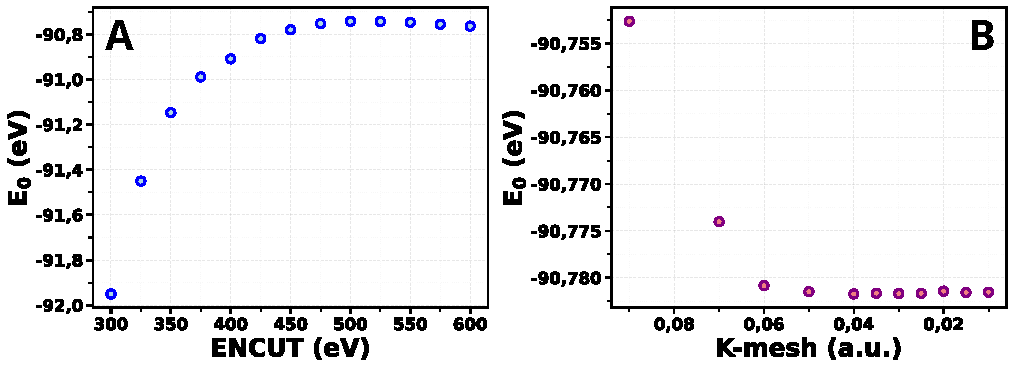
\includegraphics[width=1.0\textwidth]{figuras/graficos/convergencia_encut_kpoints.pdf}
    \fonte{Elaborada pelo autor.}
\end{figure}
\FloatBarrier

Primeiramente para a otimização do sistema foi realizada a determinação do ENCUT mínimo do sistema, que define o limite da energia cinética das funções de ondas planas que contribuirão na descrição da função de onda do sistema e com isso determinação da energia total do sistema (E$_0$). Esse parametro é de extrema importancia para descriçãoda E$_0$ e também não usar utilizar um número excessivo de funções de base que não aumentar significativamente a precisão do resultado e aumetaram o tempo de calculo, visto que acima de um valor limite a energia total do sistema tende a convergir para um valor limite. Sendo assim foram feitos calculos de relaxação do \textit{bulk} de ZnWO$_4$ variando o ENCUT de 300 a 600 eV. A partir dos resultados apresentados na Figura \ref{fig:convergencia_encut_kpoints} A observa-se que o E$_0$ do sistema converge para um valor limite a partir de um ENCUT de 450 eV, portanto esse valor foi escolhido para os cálculos subsequentes. A partir desse resultado realizou-se a determinação do número ótimo de \textit{k-points} para a amostragem da zona de Brillouin do sistema. Foram realizados cálculos variando a densidade da malha de \textit{k-points} (K-MESH) com o auxílio do \textit{vaspkit} foi gerado os \textit{k-points}, a densidade da malha foi variada de 0,01 a 0,09. A partir dos resultados apresentados na Figura \ref{fig:convergencia_encut_kpoints}B observa-se que o E$_0$ do sistema converge para um valor limite a partir de uma malha de densidade 0.04, que corresponde aos \textit{k-points} de 5x4x5, portanto esse valor foi escolhido para os cálculos subsequentes.

Feita essa otimização inicial dos parâmetros de cálculo, foi realizado um estudo do funcional de troca e correlação mais adequado para descrever o sistema, para isso foi utilizada a entalpia de formação do material como parametro de comparação. Foram testados os funcionais GGA do tipo PBE (usado até o momento), PBE revisado por Zhang e Yang (revPBE) \cite{zhang1998comment} e PBE revisado para sólidos e superfícies (PBEsol) \cite{perdew2008restoring} e PBE revisado Hammer \textit{et. al.} (RPBE) \cite{hammer1999improved} que tem como objetivo de aprimorar a descrição de energia de adsorção. A Tabela \ref{tab:entalpia_formaçao} apresenta os valores de entalpia obtidos para cada funcional testado, comparados com o valor experimental de -12,78 eV disponível na literatura \cite{dellien1976chromium}.

\FloatBarrier
\begin{table}[!htbp]
\centering
\caption{Valores de entalpia de formação do ZnWO$_4$ obtidos com diferentes funcionais de troca e correlação comparados com o valor experimental.}
\label{tab:entalpia_formaçao}
\begin{tabular}{lcc}
\hline
\textbf{Funcional} & \textbf{Entalpia de Formação (eV mol$^{-1}$)} & \textbf{Erro (\%)}
\\ \hline
PBE & -11,518 &  9,870 \\
revPBE & -10,556 & 17,40 \\
PBEsol & -11,977 & 6,280 \\
RPBE & -10,512 & 17,74 \\
Experimental \cite{dellien1976chromium} & -12,78  & - \\
\hline
\end{tabular}
\end{table}
\FloatBarrier

A partir dos resultados apresentados na Tabela \ref{tab:entalpia_formaçao} observa-se que o funcional GGA-PBEsol apresentou os valores de valor de entalpia de formação mais próximos dos valores experimentais, com um erro percentual de aproximadamente 5,86\%. Portanto, esse funcional foi escolhido para os cálculos subsequentes. 

Para terminar a otimização das estrutura do ZnWO$_4$ foi realizados calculos variando o fator de escala dos parametros de rede a fim de determinar a estrutura de mínima energia do sistema. Para isso foi feito um primeiro estudo variando o fator de escala de 0,800 a 1,300, a fim de obter uma estimativa inicial dos parametros de rede ótimos. A partir desse resultado foi realizado um segundo estudo mais refinado variando o fator de escala de 0,960 a 1,020. Os resultados desses cálculos estão apresentados na Figura \ref{fig:curva_fit_birch}.

\FloatBarrier
\begin{figure}[!htbp]
    \caption{Curva de Energia total (E$_0$) versus volume (V) do ZnWO$_4$ obtida a partir variação do fator de escala dos parametros de rede.}
    \label{fig:curva_fit_birch}
    \centering
    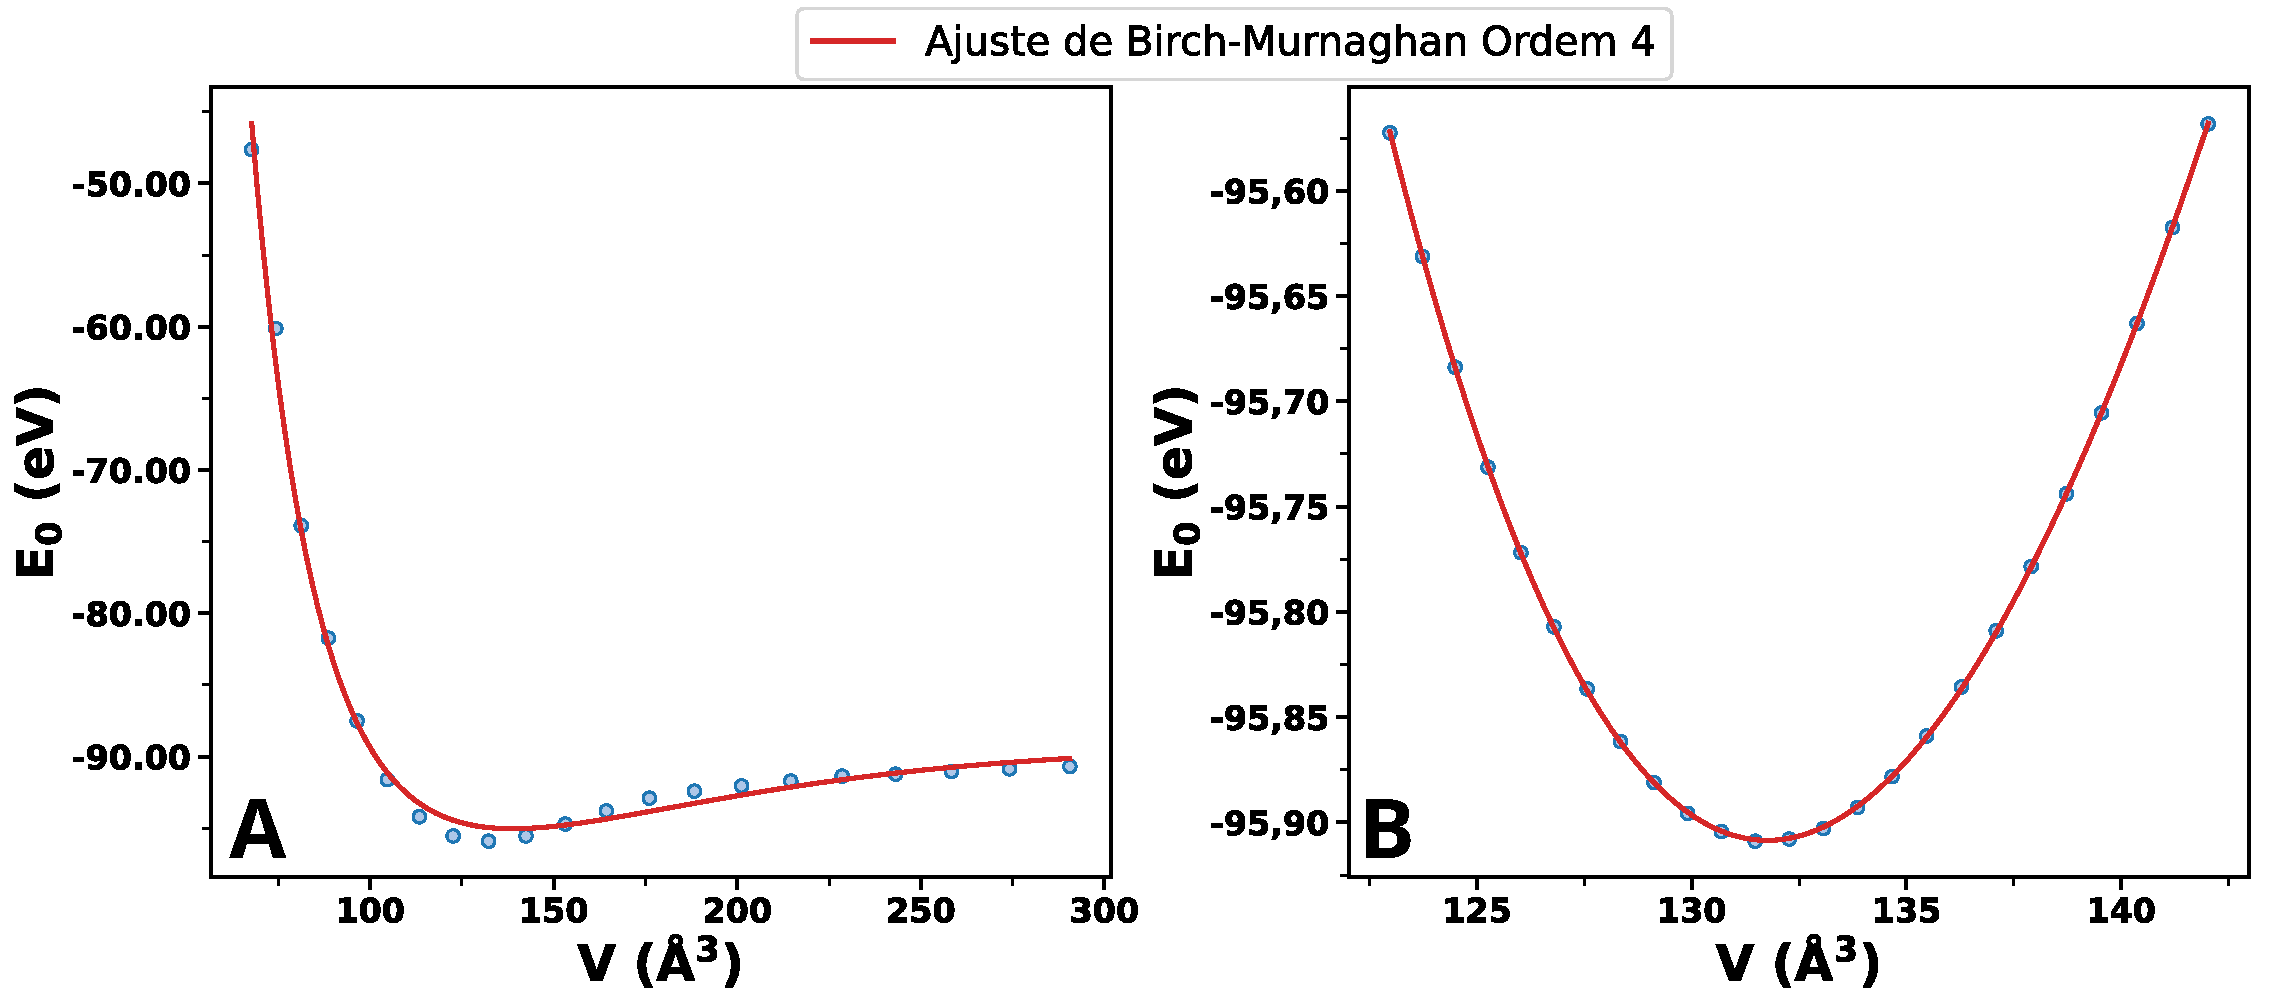
\includegraphics[width=1.0\textwidth]{figuras/graficos/curva_fit_birch.pdf}
    \fonte{Elaborada pelo autor.}
\end{figure}
\FloatBarrier

Os resultados preliminares expostos na Figura \ref{fig:curva_fit_birch}A foi observado que a energia total do sistema atinge um valor mínimo para no volume de 132,272 \AA$^3$ (fator de escala igual a 1,000). Ao realizar um estudo mais refinado com variações menores no fator de escala do parametro de rede próximo ao primeiro valor deminimo e fazendo um ajuste não linear utilizando a equação de Birch-Murnaghan foi obtida um volume mínimo de 131,480 \AA$^3$ (fator de escala igual a 0,998). Ao utilizar esse fator de escala de rede na estrutura do ZnWO$_4$ para obtenção da sua E$_0$ mínima comprovou-se que esse valor de fator de escala realmente corresponde ao valor mínimo de energia do sistema. Os parametros de rede obtido pela otimização de volume foram comparados com resultados experimentais e teóricos da literatura, para averiguar a validade dos resultados obtidos. A Tabela \ref{tab:parametros_de_rede_ZnWO4} os parametros de rede obtidos em comparativo com a literatura para o ZnWO$_4$.

\FloatBarrier
\begin{table}[!htbp]
\centering
\caption{Parametros de rede do ZnWO$_4$ frente ao literatura.}
\label{tab:parametros_de_rede_ZnWO4}
\begin{tabular}{lccc p{5cm}}
\hline
\textbf{Natureza do resultado} & \textbf{a} & \textbf{b} & \textbf{c} & \textbf{Referência}
\\ \hline
Calculado & 4,6674 & 5,7182 & 4,9364 & Presente trabalho \\
Calculado &  4.702 &  5.755 & 4.917 & Hoang (2018) \cite{hoang2018electronic} \\
Calculado & 4.736 & 5.746 & 4.937 & Zhang (2023) \cite{zhang2023effect} \\
Experimental & 4.6849 & 5.7172 & 4.9328 & Dkhilalli \textit{et. al.} (2018) \cite{dkhilalli2018structural} \\
Experimental &  4.691 & 5.720 &  4.925 & Yan \textit{et. al.} (2019) \cite{yan2019study} \\

\hline
\end{tabular}
\end{table}
\FloatBarrier

Ao comparar os resultados obtidos com a literatura foi observado um elevada similaridade entre os resultados. O que serve de indicativo de que o modelo construido apresnta boa representatividade estrutural do material.

Uma vez estabelecida o ENCUT, \textit{k-points}, funcional de troca correlação e parametros de rede que melhor descrevem do ZnWO$_4$ pode-se avançar para construção de possíveis terminações superfíciais do material bem como o estudo de suas estabilidade segundo a Termodinâmica Atomística de Primeiros Princípios \cite{reuter2005ab,rogal2006}.

\subsection{Construção das superfícies e estudo de estabilidade}
A partir da estrutura otimizada do ZnWO$_4$ foram construídas as superfícies de baixos índices de Miller (001), (010), (011), (100), (101) (110) e (111). \textcolor{red}{Essas superfícies foram escolhidas por serem as mais prováveis de serem expostas em cristais do material, conforme observado em estudos experimentais \cite{pereira2018znwo}}. Para cada orientação foram geradas diferentes terminações superficiais, de 15 \AA de espessura e com um vácuo de 15 \AA, totalizando 50 terminações. A Tabela \ref{tab:terminações_znwo4} apresenta o número terminações superficiais geradas para cada orientação e suas respectivas identificações.

\FloatBarrier
\begin{table}[!htbp]
\centering
\caption{Terminações superficiais geradas para cada orientação do ZnWO$_4$.}
\label{tab:terminações_znwo4}
\begin{tabular}{lcc}
\hline
\textbf{Orientação} & \textbf{Identificação} & \textbf{Número de Terminações}
\\ \hline
(001) & ST-A & 5 \\
(010) & ST-B & 8 \\
(011) & ST-C & 12 \\
(100) & ST-D & 6 \\
(101) & ST-E & 3 \\
(110) & ST-F & 8 \\
(111) & ST-G & 8 \\
\hline
\end{tabular}
\end{table}
\FloatBarrier

Os \textit{slabs} referentes as terminações geradas para cada superficies tiveram sua estabilidade avaliada por meio do calculo de energia livre de superfície ($\gamma$) segundo a Equação \ref{eq:gibbs_superficie_final}, com o auxílio da plataforma de automatização de calculos PS-TEROS. A partir dessa equação é possível avaliar a estabilidade de diferentes terminações de forma comparativa de duas maneiras. Primeiro traçando um diagrama de energia em que é estabelecida uma condição de potencial químico do cátion metálico modificador de rede (neste caso definindo como zero) e calculando a energia livre de superfície em função do potencial químico do oxigênio, permitindo assim identificar qual terminação é mais estável para uma determinada condição de ambiente químico. A segunda maneira é traçando um diagrama de estabilidade das terminações em que varia-se tanto o potencial químico do oxigênio quanto o do cátion metálico modificador da rede, permitindo assim identificar quais terminações são termodinamicamente mais estáveis sob diferentes condições de ambiente químico. Também é posssível relacionar a temperatura e pressão do ambiente químico com os potenciais químicos do oxigênio (Equação \ref{eq:delta_mu_o_temp_press}), permitindo assim estabelecer condições experimentais para a obtenção de determinadas terminações superficiais.



\subsubsection{Estudo de estabilidade superfície (001)}

Para a orientação (001) foram geradas 5 terminações superficiais diferentes, identificadas como ST-A1 a ST-A5. A Figura \ref{fig:znwo4_superficie_001} apresenta as estruturas das diferentes terminações superficiais geradas para essa orientação, antes e após a relaxação das estruturas, bem como seus defeitos estruturais.

\FloatBarrier
\begin{figure}[!htbp]
    \caption{Estruturas das diferentes terminações superficiais (001) do ZnWO$_4$: (A) ST-A1, (B) ST-A2, (C) ST-A3, (D) ST-A4 e (E) ST-A5, antes e após a relaxação das estruturas.}
    \label{fig:znwo4_superficie_001}
    \centering
    
\includegraphics[width=0.50\textwidth]{figuras/imagens/exemplo.jpg}
    \fonte{Elaborada pelo autor.}
\end{figure}
\FloatBarrier

A partir dos E$_0$ obtidos para cada terminação superficial, foi possível $\gamma$ em função de $\Delta \mu_O$ e também foi possível gerar o diagrama de superfície que relaciona o $\mu_O$ com $\Delta \mu_Zn$. Os resultados desses cálculos estão apresentados na Figura \ref{fig:energia_superficie_001}.

\FloatBarrier
\begin{figure}[!htbp]
    \caption{(A) $\gamma$ em função de $\Delta \mu_O$ para as diferentes terminações superficiais (001) do ZnWO$_4$. (B) Diagrama de estabilidade das terminações superficiais (001) em função dos potenciais químicos do oxigênio $\Delta \mu_O$ e $\Delta \mu_{Zn}$. (C) Relação de T para diferentes $\Delta \mu_O$ e pressões parciais de O$_2$.}
    \label{fig:energia_superficie_001}
    \centering
    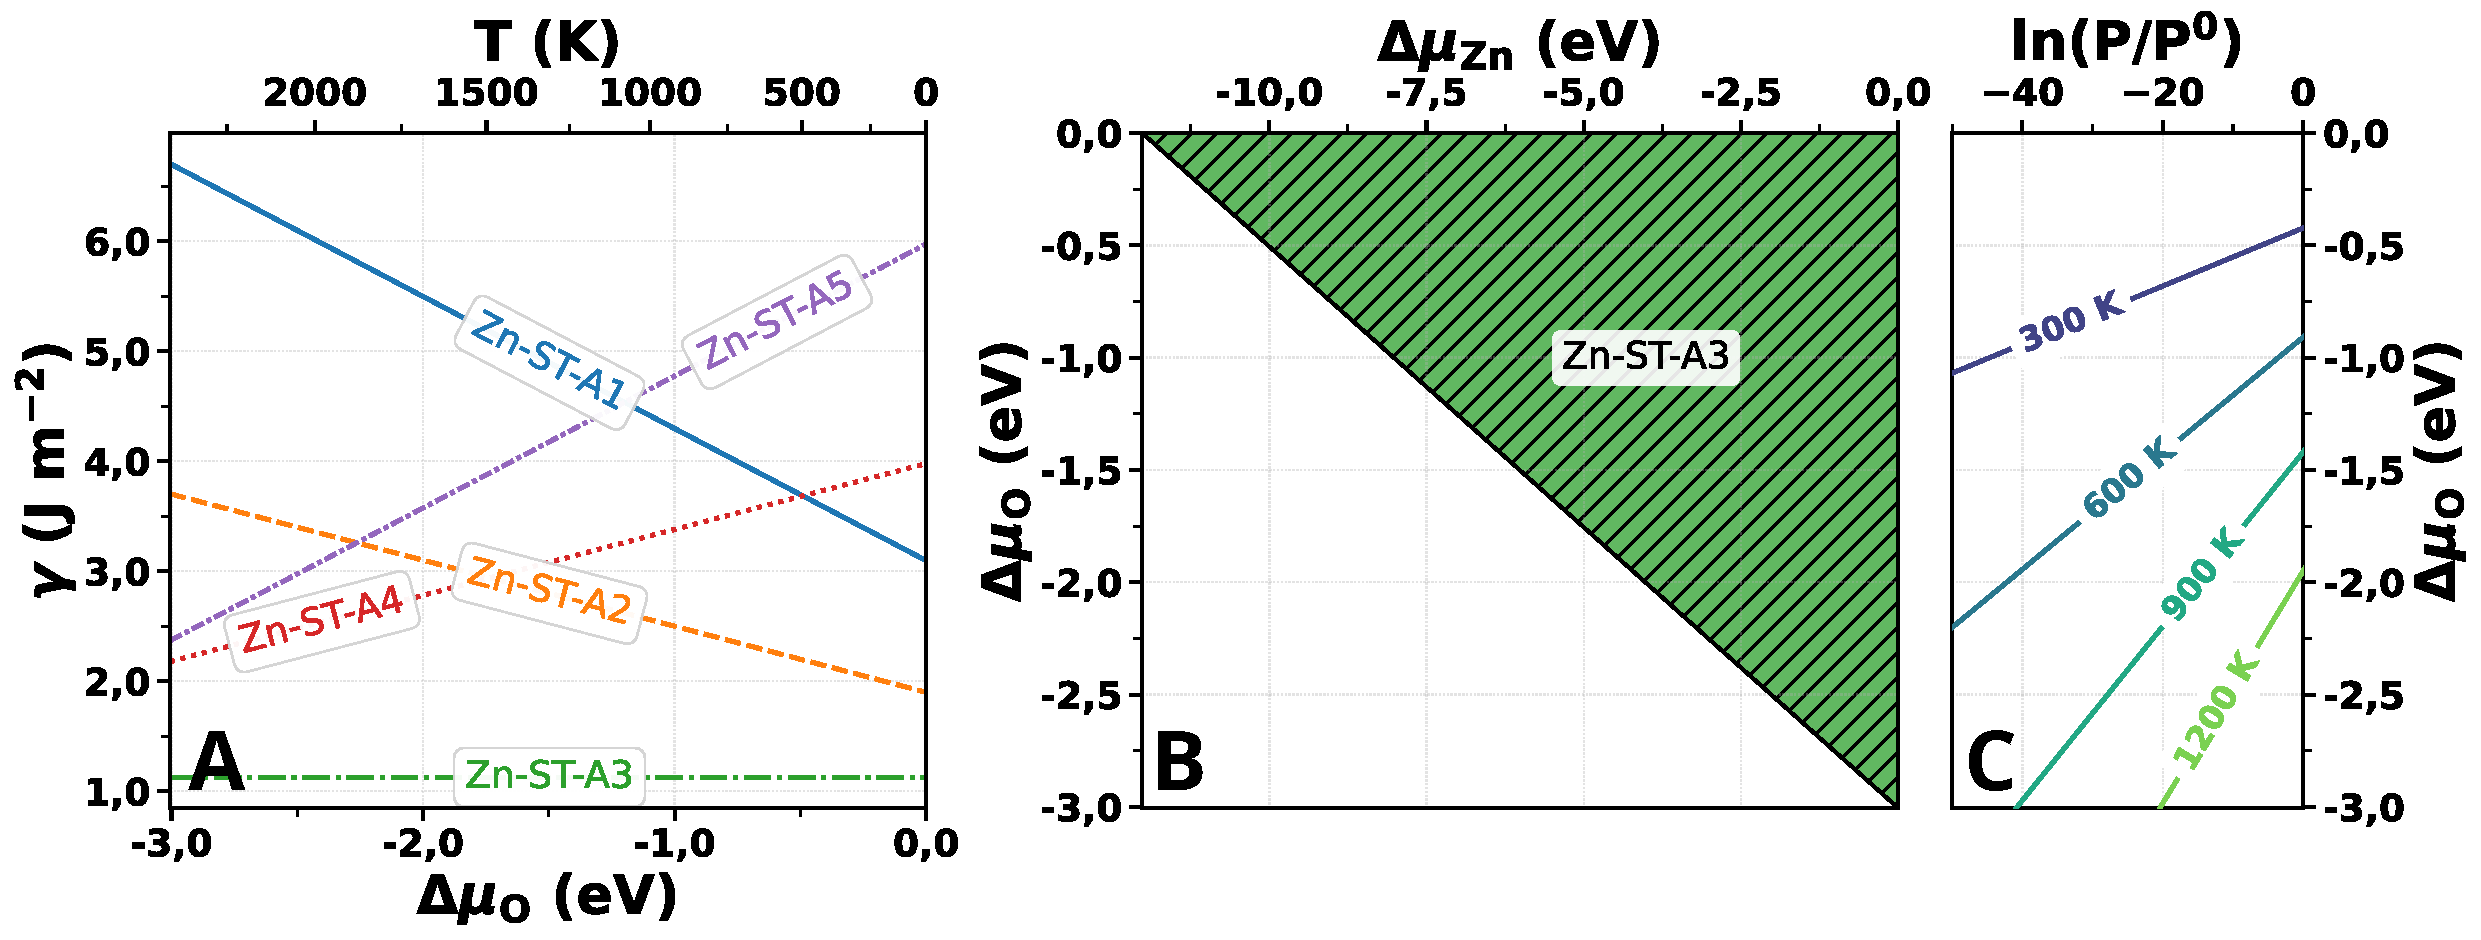
\includegraphics[width=1.0\textwidth]{figuras/graficos/energia_superficie_001.pdf}
    \fonte{Elaborada pelo autor.}
\end{figure}
\FloatBarrier

\subsubsection{Estudo de estabilidade superfície (010)}
Para a orientação (010) foram geradas 8 terminações superficiais diferentes, identificadas como ST-B1 a ST-B8. A Figura \ref{fig:znwo4_superficie_010} apresenta as estruturas das diferentes terminações superficiais geradas para essa orientação, antes e após a relaxação das estruturas, bem como seus defeitos estruturais.

\FloatBarrier
\begin{figure}[!htbp]
    \caption{Estruturas das diferentes terminações superficiais (010) do ZnWO$_4$: (A) ST-B1, (B) ST-B2, (C) ST-B3, (D) ST-B4, (E) ST-B5, (F) ST-B6, (G) ST-B7 e (H) ST-B8, antes e após a relaxação das estruturas.}
    \label{fig:znwo4_superficie_010}
    \centering
    
\includegraphics[width=0.50\textwidth]{figuras/imagens/exemplo.jpg}
    \fonte{Elaborada pelo autor.}
\end{figure}
\FloatBarrier

A partir dos E$_0$ obtidos para cada terminação superficial, foi possível calcular $\gamma$ em função de $\Delta \mu_O$. Também foi possível gerar o diagrama de superfície que relaciona o $\Delta \mu_O$ com $\Delta \mu_{Zn}$. Os resultados desses cálculos estão apresentados na Figura \ref{fig:energia_superficie_010}.

\FloatBarrier
\begin{figure}[!htbp]
    \caption{(A) $\gamma$ em função de $\Delta \mu_O$ para as diferentes terminações superficiais (010) do ZnWO$_4$ (B) Diagrama de estabilidade das terminações superficiais (010) em função de $\Delta \mu_O$ e $\Delta \mu_{Zn}$. (C) Relação de T para diferentes $\Delta \mu_O$ e pressões parciais de O$_2$.}
    \label{fig:energia_superficie_010}
    \centering
    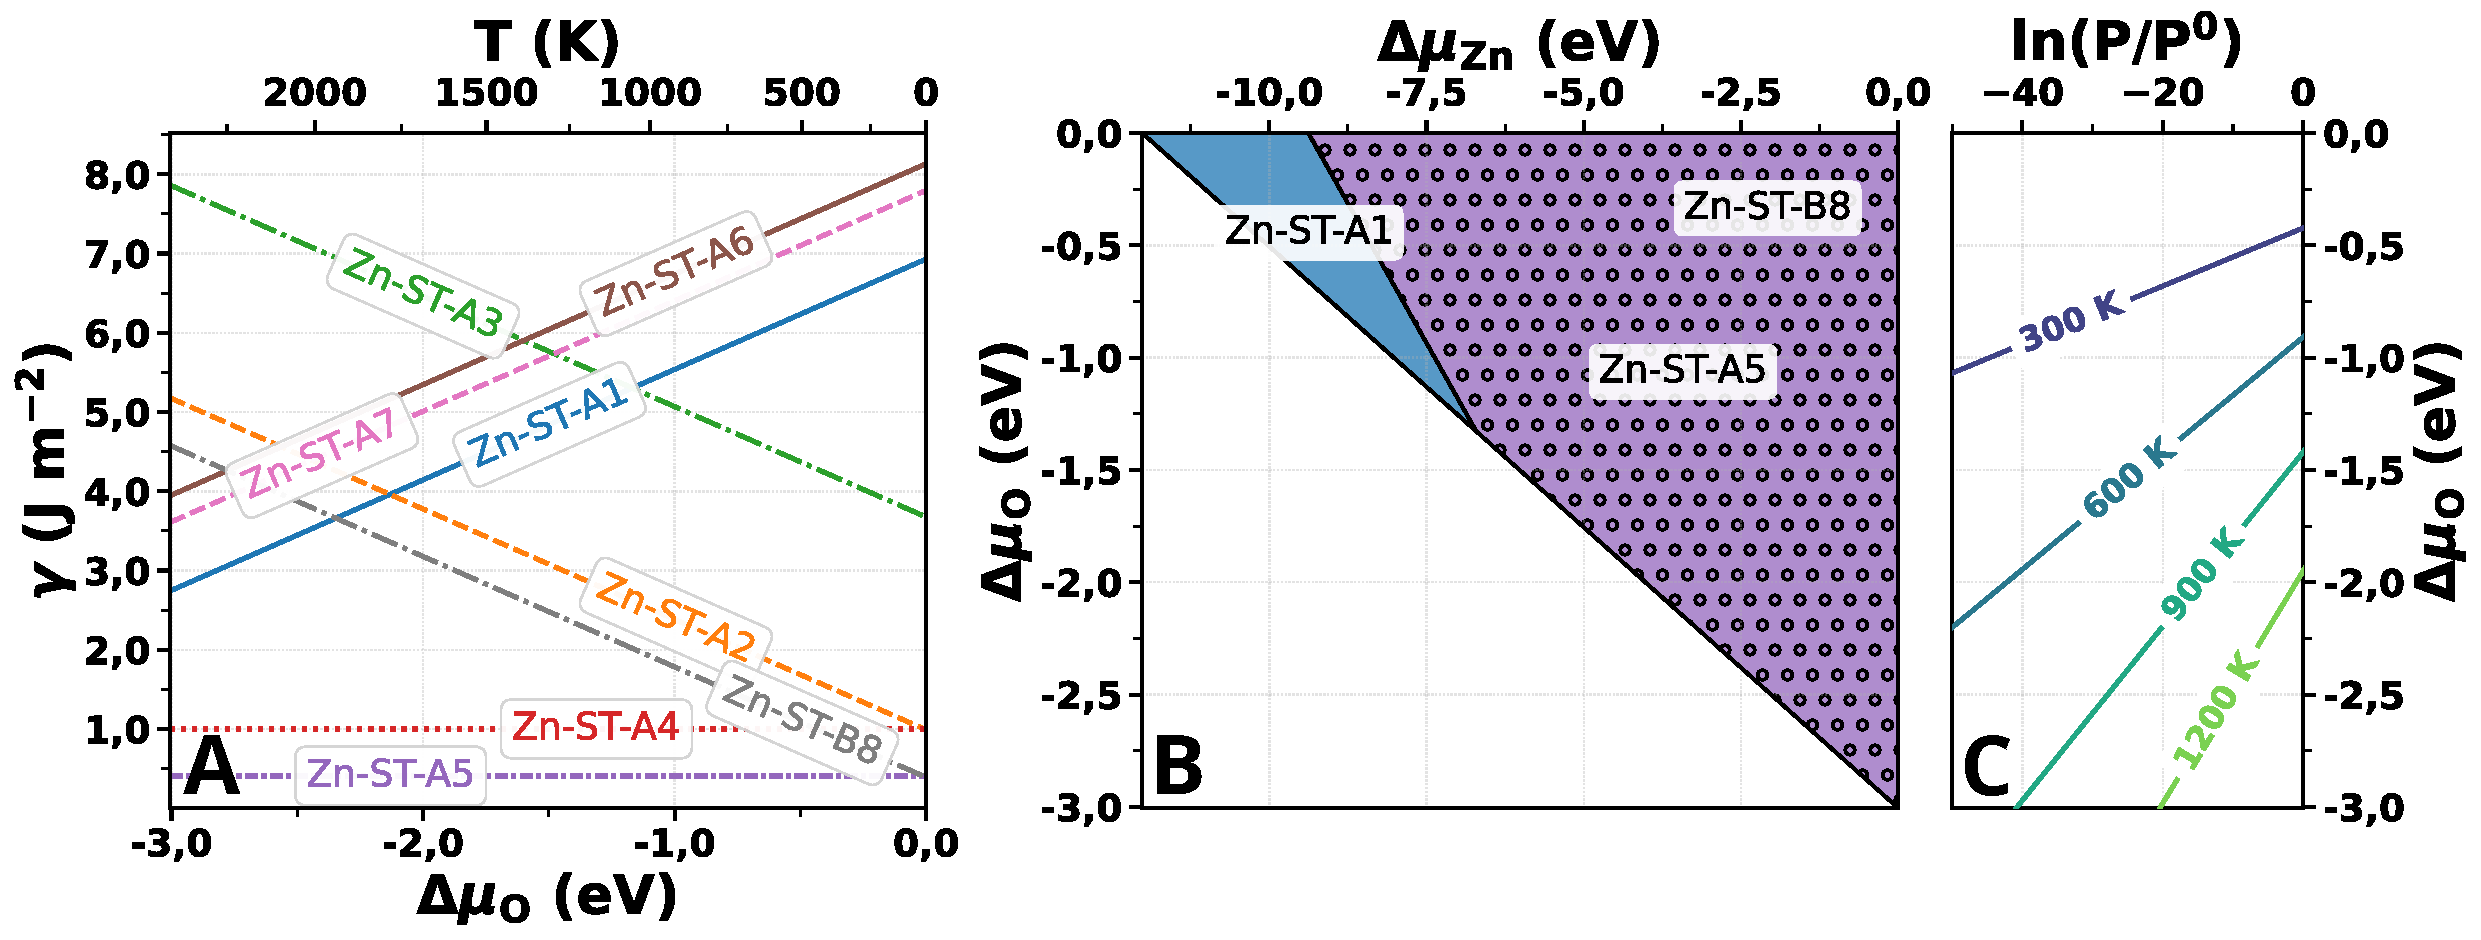
\includegraphics[width=1.0\textwidth]{figuras/graficos/energia_superficie_010.pdf}
    \fonte{Elaborada pelo autor.}
\end{figure}
\FloatBarrier

\subsubsection{Estudo de estabilidade superfície (011)}
Para a orientação (011) foram geradas 12 terminações superficiais diferentes, identificadas como ST-C1 a ST-C12. A Figura \ref{fig:znwo4_superficie_011} apresenta as estruturas das diferentes terminações superficiais geradas para essa orientação, antes e após a relaxação das estruturas, bem como seus defeitos estruturais.

\FloatBarrier
\begin{figure}[!htbp]
    \caption{Estruturas das diferentes terminações superficiais (011) do ZnWO$_4$: (A) ST-C1, (B) ST-C2, (C) ST-C3, (D) ST-C4, (E) ST-C5, (F) ST-C6, (G) ST-C7, (H) ST-C8, (I) ST-C9, (J) ST-C10, (K) ST-C11 e (L) ST-C12, antes e após a relaxação das estruturas.}
    \label{fig:znwo4_superficie_011}
    \centering
    
\includegraphics[width=0.50\textwidth]{figuras/imagens/exemplo.jpg}
    \fonte{Elaborada pelo autor.}
\end{figure}
\FloatBarrier


\subsubsection{Estudo de estabilidade superfície (100)}
Para a orientação (100) foram geradas 6 terminações superficiais diferentes, identificadas como ST-D1 a ST-D6. A Figura \ref{fig:znwo4_superficie_100} apresenta as estruturas das diferentes terminações superficiais geradas para essa orientação, antes e após a relaxação das estruturas, bem como seus defeitos estruturais.

\FloatBarrier
\begin{figure}[!htbp]
    \caption{Estruturas das diferentes terminações superficiais (100) do ZnWO$_4$: (A) ST-D1, (B) ST-D2, (C) ST-D3, (D) ST-D4, (E) ST-D5 e (F) ST-D6, antes e após a relaxação das estruturas, bem como seus defeitos estruturais.}
    \label{fig:znwo4_superficie_100}
    \centering
    
\includegraphics[width=0.50\textwidth]{figuras/imagens/exemplo.jpg}
    \fonte{Elaborada pelo autor.}
\end{figure}
\FloatBarrier

A partir dos E$_0$ obtidos para cada terminação superficial, foi possível calcular $\gamma$ em função de $\Delta \mu_O$. Também foi possível gerar o diagrama de superfície que relaciona o $\Delta \mu_O$ com $\Delta \mu_{Zn}$. Os resultados desses cálculos estão apresentados na Figura \ref{fig:energia_superficie_100}.

\FloatBarrier
\begin{figure}[!htbp]
    \caption{(A) $\gamma$ em função de $\Delta \mu_O$ para as diferentes terminações superficiais (100) do ZnWO$_4$ (B) Diagrama de estabilidade das terminações superficiais (100) em função de $\Delta \mu_O$ e $\Delta \mu_{Zn}$. (C) Relação de T para diferentes $\Delta \mu_O$ e pressões parciais de O$_2$.}
    \label{fig:energia_superficie_100}
    \centering
    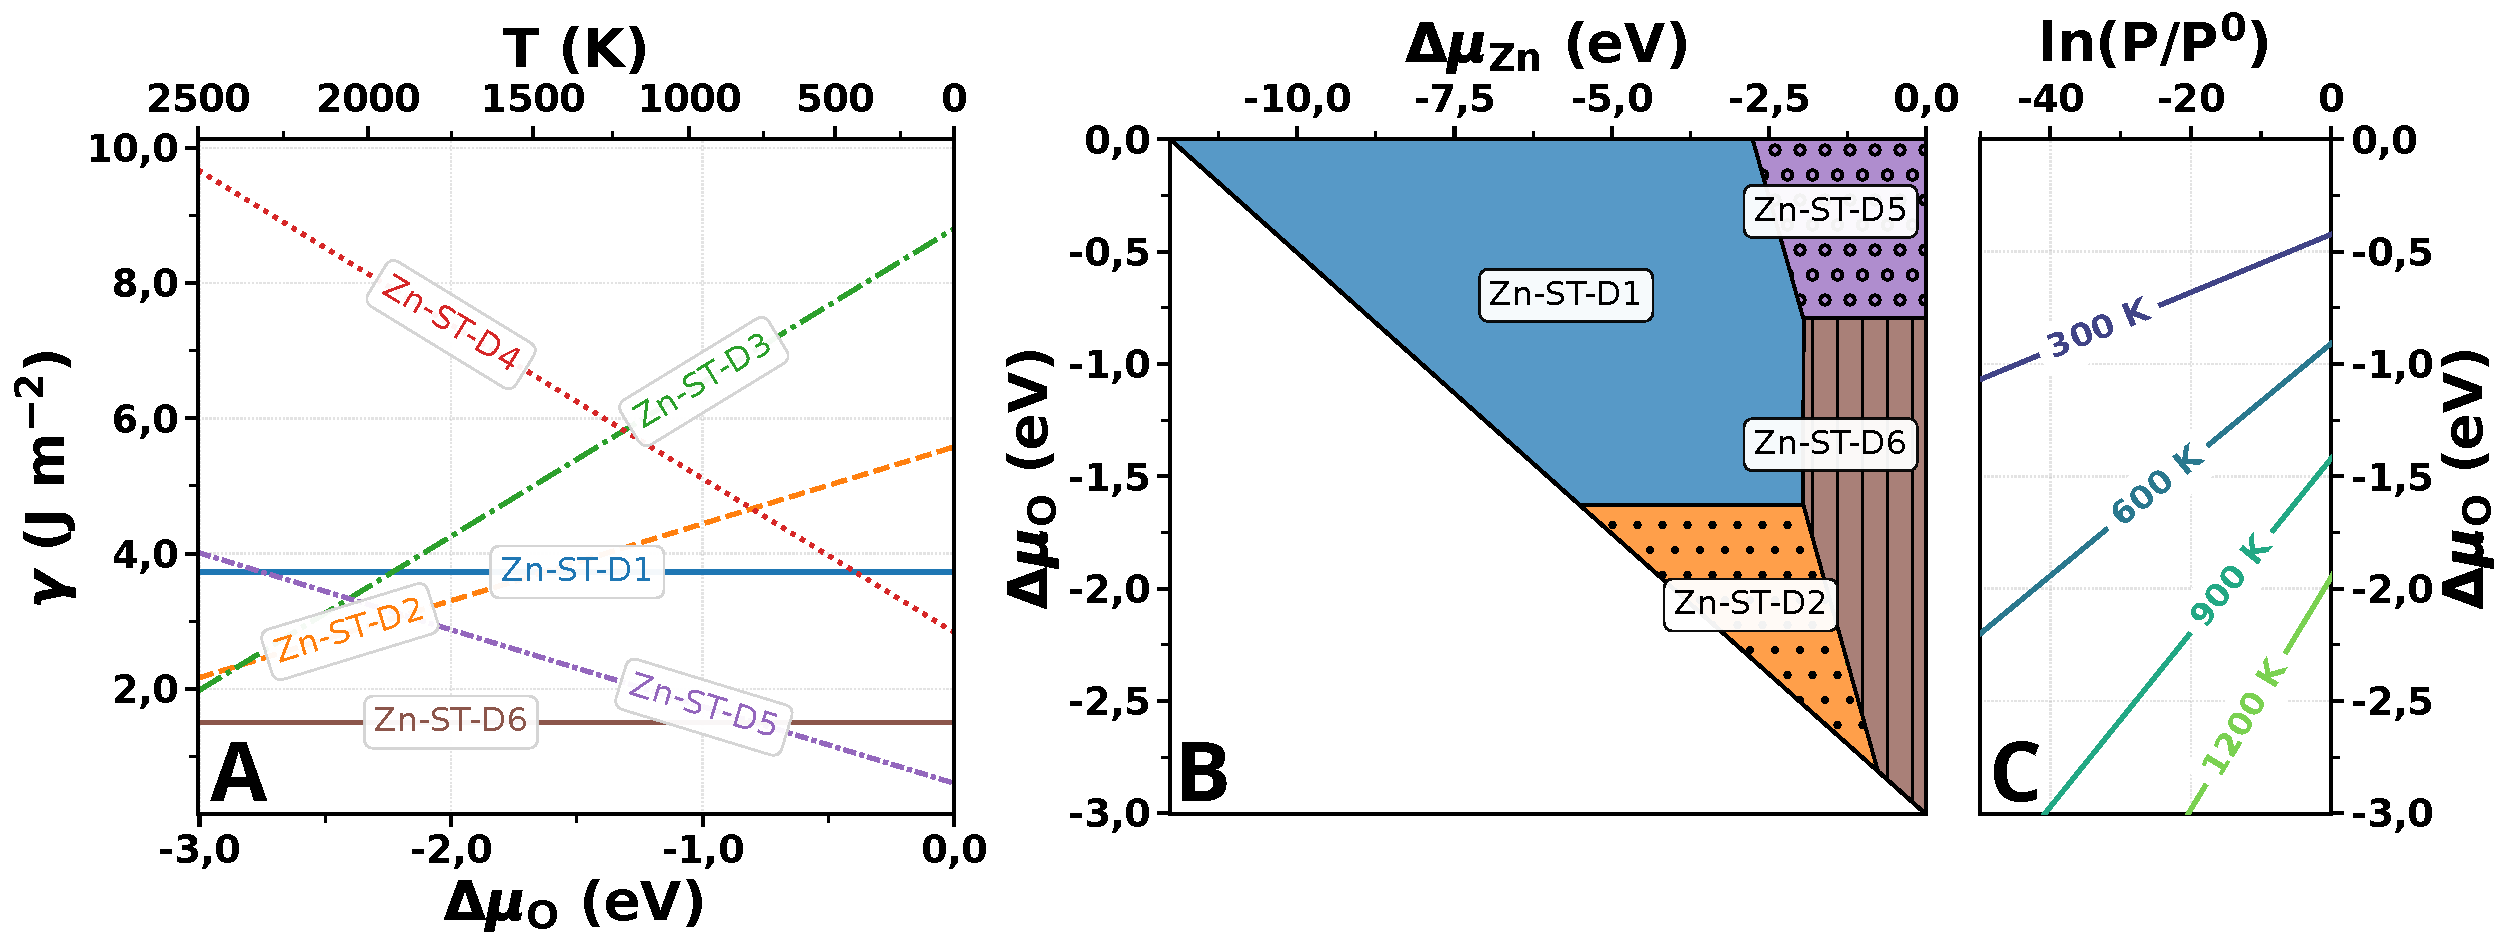
\includegraphics[width=1.0\textwidth]{figuras/graficos/energia_superficie_100.pdf}
    \fonte{Elaborada pelo autor.}
\end{figure}
\FloatBarrier

\subsubsection{Estudo de estabilidade superfície (101)}
Para a orientação (101) foram geradas 3 terminações superficiais diferentes, identificadas como ST-E1, ST-E2 e ST-E3. A Figura \ref{fig:znwo4_superficie_101} apresenta as estruturas das diferentes terminações superficiais geradas para essa orientação, antes e após a relaxação das estruturas, bem como seus defeitos estruturais.

\FloatBarrier
\begin{figure}[!htbp]
    \caption{Estruturas das diferentes terminações superficiais (101) do ZnWO$_4$: (A) ST-E1, (B) ST-E2 e (C) ST-E3, antes e após a relaxação das estruturas.}
    \label{fig:znwo4_superficie_101}
    \centering
    
\includegraphics[width=0.50\textwidth]{figuras/imagens/exemplo.jpg}
    \fonte{Elaborada pelo autor.}
\end{figure}
\FloatBarrier

A partir dos E$_0$ obtidos para cada terminação superficial, foi possível calcular $\gamma$ em função de $\Delta \mu_O$. Também foi possível gerar o diagrama de superfície que relaciona o $\Delta \mu_O$ com $\Delta \mu_{Zn}$. Os resultados desses cálculos estão apresentados na Figura \ref{fig:energia_superficie_101}.

\FloatBarrier
\begin{figure}[!htbp]
    \caption{(A) $\gamma$ em função de $\Delta \mu_O$ para as diferentes terminações superficiais (101) do ZnWO$_4$ (B) Diagrama de estabilidade das terminações superficiais (101) em função de $\Delta \mu_O$ e $\Delta \mu_{Zn}$. (C) Relação de T para diferentes $\Delta \mu_O$ e pressões parciais de O$_2$.}
    \label{fig:energia_superficie_101}
    \centering
    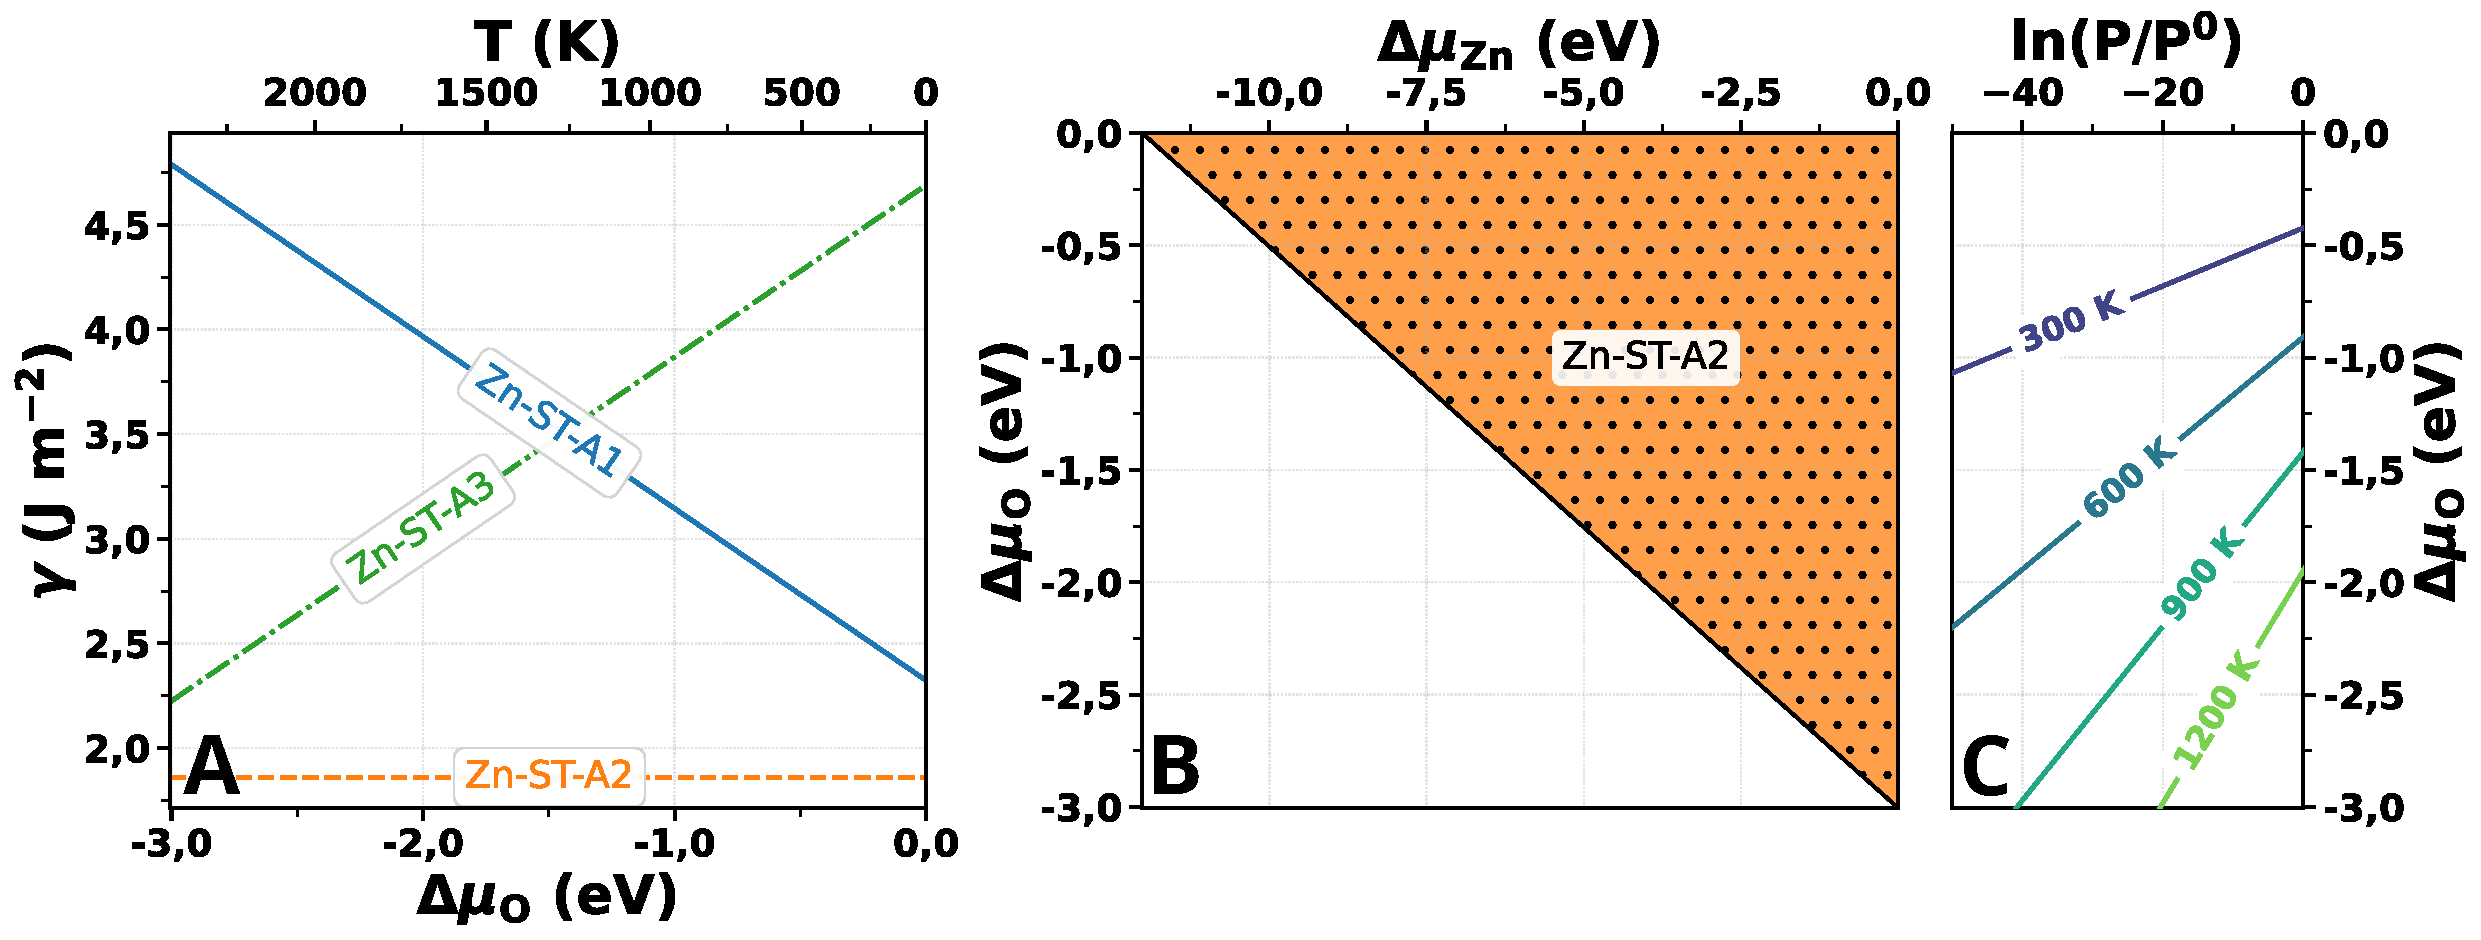
\includegraphics[width=1.0\textwidth]{figuras/graficos/energia_superficie_101.pdf}
    \fonte{Elaborada pelo autor.}
\end{figure}
\FloatBarrier

\subsubsection{Estudo de estabilidade superfície (110)}
Para a orientação (110) foram geradas 8 terminações superficiais diferentes, identificadas como ST-F1 a ST-F8. A Figura \ref{fig:znwo4_superficie_110} apresenta as estruturas das diferentes terminações superficiais geradas para essa orientação, antes e após a relaxação das estruturas, bem como seus defeitos estruturais.

\FloatBarrier
\begin{figure}[!htbp]
    \caption{Estruturas das diferentes terminações superficiais (110) do ZnWO$_4$: (A) ST-F1, (B) ST-F2, (C) ST-F3, (D) ST-F4, (E) ST-F5, (F) ST-F6, (G) ST-F7 e (H) ST-F8, antes e após a relaxação das estruturas.}
    \label{fig:znwo4_superficie_110}
    \centering
    
\includegraphics[width=0.50\textwidth]{figuras/imagens/exemplo.jpg}
    \fonte{Elaborada pelo autor.}
\end{figure}
\FloatBarrier

A partir dos E$_0$ obtidos para cada terminação superficial, foi possível calcular $\gamma$ em função de $\Delta \mu_O$. Também foi possível gerar o diagrama de superfície que relaciona o $\Delta \mu_O$ com $\Delta \mu_{Zn}$. Os resultados desses cálculos estão apresentados na Figura \ref{fig:energia_superficie_110}.

\FloatBarrier
\begin{figure}[!htbp]
    \caption{(A) $\gamma$ em função de $\Delta \mu_O$ para as diferentes terminações superficiais (110) do ZnWO$_4$ (B) Diagrama de estabilidade das terminações superficiais (110) em função de $\Delta \mu_O$ e $\Delta \mu_{Zn}$. (C) Relação de T para diferentes $\Delta \mu_O$ e pressões parciais de O$_2$.}
    \label{fig:energia_superficie_110}
    \centering
    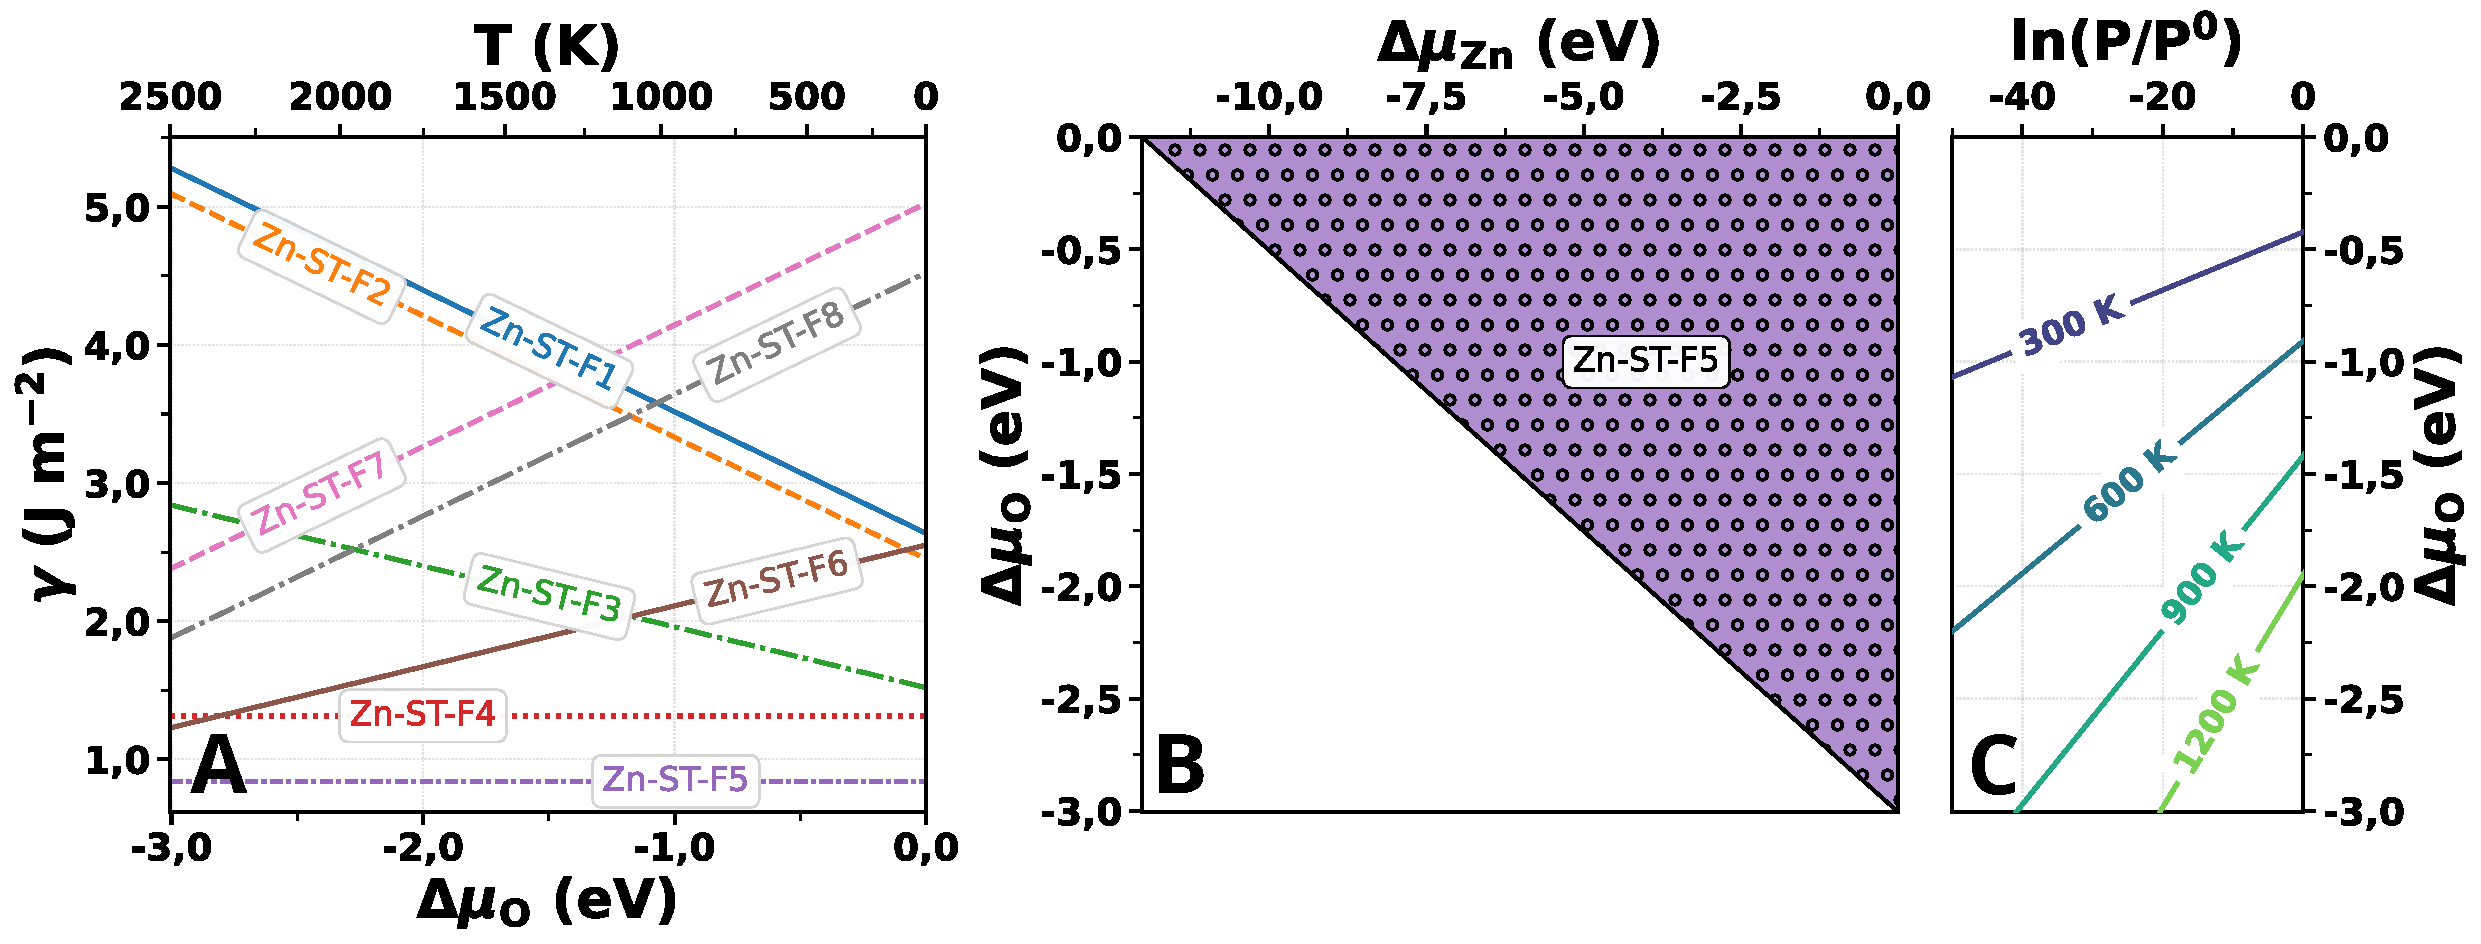
\includegraphics[width=1.0\textwidth]{figuras/graficos/energia_superficie_110.pdf}
    \fonte{Elaborada pelo autor.}
\end{figure}
\FloatBarrier

\subsubsection{Estudo de estabilidade superfície (111)}
Por fim para a orientação (111) foram geradas 8 terminações superficiais diferentes, identificadas como ST-G1 a ST-G8. A Figura \ref{fig:znwo4_superficie_111} apresenta as estruturas das diferentes terminações superficiais geradas para essa orientação, antes e após a relaxação das estruturas, bem como seus defeitos estruturais.

\FloatBarrier
\begin{figure}[!htbp]
    \caption{Estruturas das diferentes terminações superficiais (111) do ZnWO$_4$: (A) ST-G1, (B) ST-G2, (C) ST-G3, (D) ST-G4, (E) ST-G5, (F) ST-G6, (G) ST-G7 e (H) ST-G8, antes e após a relaxação das estruturas.}
    \label{fig:znwo4_superficie_111}
    \centering
    
\includegraphics[width=0.50\textwidth]{figuras/imagens/exemplo.jpg}
    \fonte{Elaborada pelo autor.}
\end{figure}
\FloatBarrier

% Inclua figuras e tabelas conforme necessário.

\fi
\ifincluirconclusao
% 6_conclusao.tex
\chapter{CONCLUSÃO}

Sintetize as principais contribuições do trabalho, tire conclusões a partir dos resultados e proponha trabalhos futuros.


\fi

\ifincluirreferencias
% ===== Referências =====
\clearpage
\cleardoublepage
\phantomsection
% Definir tamanho da fonte 14 para a seção de referências
{\fontsize{14}{16}\selectfont
\printbibliography[title={REFERÊNCIAS},heading=bibintoc]
}
\fi

\ifincluirapendice
% ===== Apêndice =====
\clearpage
\cleardoublepage
% O apêndice é incluído após as referências
% Os capítulos do apêndice usam \chapter* para não serem numerados
% e \addcontentsline para aparecerem no sumário sem numeração
% apendice.tex
% Apêndice do projeto de doutorado

% Apêndice A - Título do Apêndice A
\chapter*{APÊNDICE A -- Título do Apêndice A}
\addcontentsline{toc}{chapter}{APÊNDICE A -- Título do Apêndice A}

\begin{mytext}

Este é o conteúdo do apêndice A. Você pode incluir materiais suplementares, derivações matemáticas detalhadas, códigos computacionais, ou qualquer outro conteúdo que complemente o trabalho principal.

\lipsum[1-2]

\end{mytext}

% Apêndice B - Título do Apêndice B
\chapter*{APÊNDICE B -- Título do Apêndice B}
\addcontentsline{toc}{chapter}{APÊNDICE B -- Título do Apêndice B}

\begin{mytext}

Este é o conteúdo do apêndice B. Você pode adicionar mais seções conforme necessário.

\lipsum[3-4]

\end{mytext}

% Adicione mais apêndices conforme necessário
% \chapter*{APÊNDICE C -- Título do Apêndice C}
% \addcontentsline{toc}{chapter}{APÊNDICE C -- Título do Apêndice C}
% 
% \begin{mytext}
% Conteúdo do apêndice C...
% \end{mytext}

\fi

\end{document}
